\documentclass[11pt]{article}

\usepackage{tocloft}
\usepackage[margin=1in]{geometry} %used for margins
\usepackage{graphics}
\usepackage{graphicx}
\usepackage{gensymb} %for symbols such as the degree sign
\usepackage{titlesec}
\graphicspath{
{figures/}
{../figures/}
{../../figures/}
{../../figures/plots/}
{../../figures/screenshots/}
{../../figures/diagrams/experiment_1/}
{../../../figures/}
}
\usepackage[natbibapa]{apacite}
\usepackage{xcolor}
\usepackage{array}% http://ctan.org/pkg/array
\usepackage{bibentry} %for full citations
% \nobibliography* 
\usepackage{subfig} %for creating panels
\usepackage{todonotes}  
\usepackage{booktabs}% http://ctan.org/pkg/booktabs
\usepackage[countmax]{subfloat} %for creating panels
\usepackage{enumitem} %better environment for lists 
\usepackage{multirow} %to have multiple row entries in tables 
\usepackage{breakurl} %to break urls
\usepackage{wrapfig} %to wrap figures
\usepackage{float}  %for floating figures
\usepackage{amsmath}
\usepackage{hyperref} %to h ave links within the document 
\hypersetup{
    colorlinks,%
    citecolor=black,%
    filecolor=black,%
    linkcolor=black,%
    urlcolor=black
}

%to allow for more figures per page 
\renewcommand\floatpagefraction{.95}
\renewcommand\topfraction{.95}
\renewcommand\bottomfraction{.95}
\renewcommand\textfraction{.05}   
\setcounter{totalnumber}{50}
\setcounter{topnumber}{50}
\setcounter{bottomnumber}{50}

%some settings to make lists look nicer 
\setlist{leftmargin=*} 
\setlist[1]{labelindent=\parindent} % Only the level 1
\setlist{topsep = 0cm,partopsep = 1pt, parsep = 1pt} %changes the separation of lists 

%some stuff to decrease the space around section headings, etc. 
\titleformat{\section}
  {\bfseries \Large}{\thesection}{0.5em}{}
\titleformat{\subsection}
  {\bfseries \large}{\thesubsection}{0.5em}{}
\titleformat{\subsubsection}
{\bfseries}{\thesubsubsection}{0.5em}{}
\titlespacing{\section}{0cm}{0.3cm}{0.1cm}
\titlespacing{\subsection}{0cm}{0.3cm}{0.1cm}
\titlespacing{\subsubsection}{0cm}{0.3cm}{0.1cm}

\begin{document}

\begin{center} 
{\LARGE \textbf{Unpacking responsibility}}
\linebreak
\linebreak
{\large Nathalie Fernandez (\href{mailto:nfern@mit.edu}{nfern@mit.edu})}
\linebreak
\today
\end{center} 

\tableofcontents 
\clearpage 

\section{To do}
\label{sec:to_do}

\begin{itemize}
	\item list of things that still need to be done ... 
\end{itemize}

\clearpage 
\section{Research question}
\label{sec:research_question}

\section{Experiment 1}
\label{sec:experiment_1}

\subsection{Methods}
\label{sub:methods}

\subsubsection{Participants}
\label{ssub:participants}

\subsubsection{Design}
\label{ssub:design}

\begin{figure}[H]
\renewcommand{\thesubfigure}{\arabic{subfigure}}
\centering
{\hfill}
\subfloat[][]{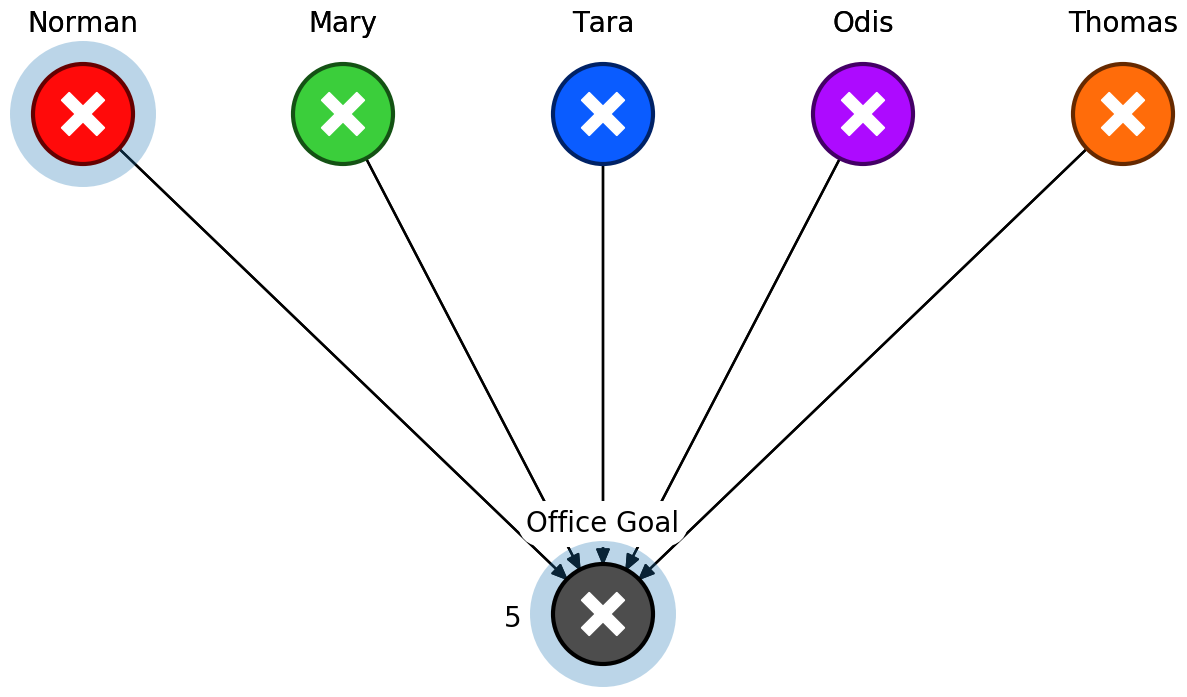
\includegraphics[width=0.22\columnwidth]{situation0}}
\hfill
\subfloat[][]{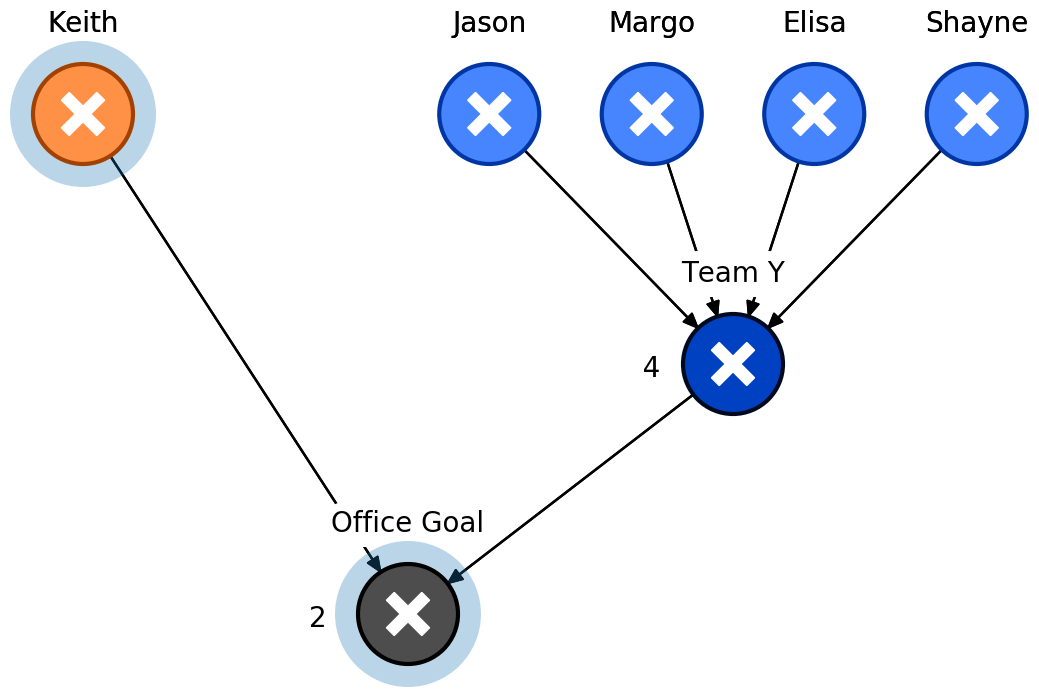
\includegraphics[width=0.22\columnwidth]{situation1}}
\hfill
\subfloat[][]{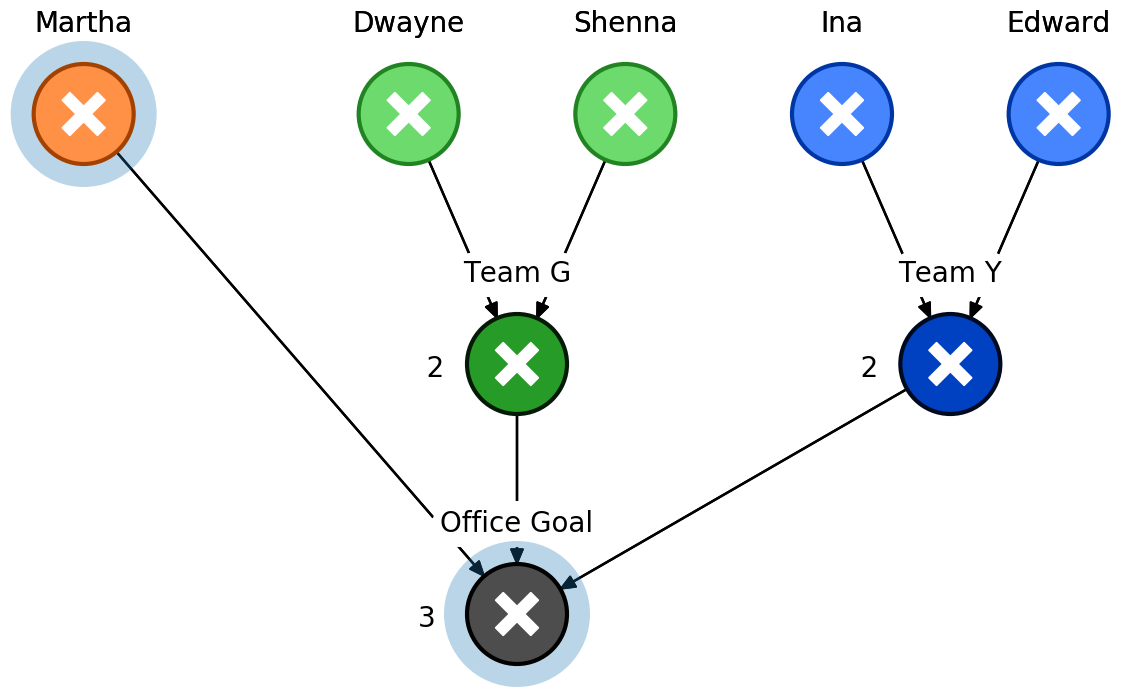
\includegraphics[width=0.22\columnwidth]{situation2}}
\hfill
\subfloat[][]{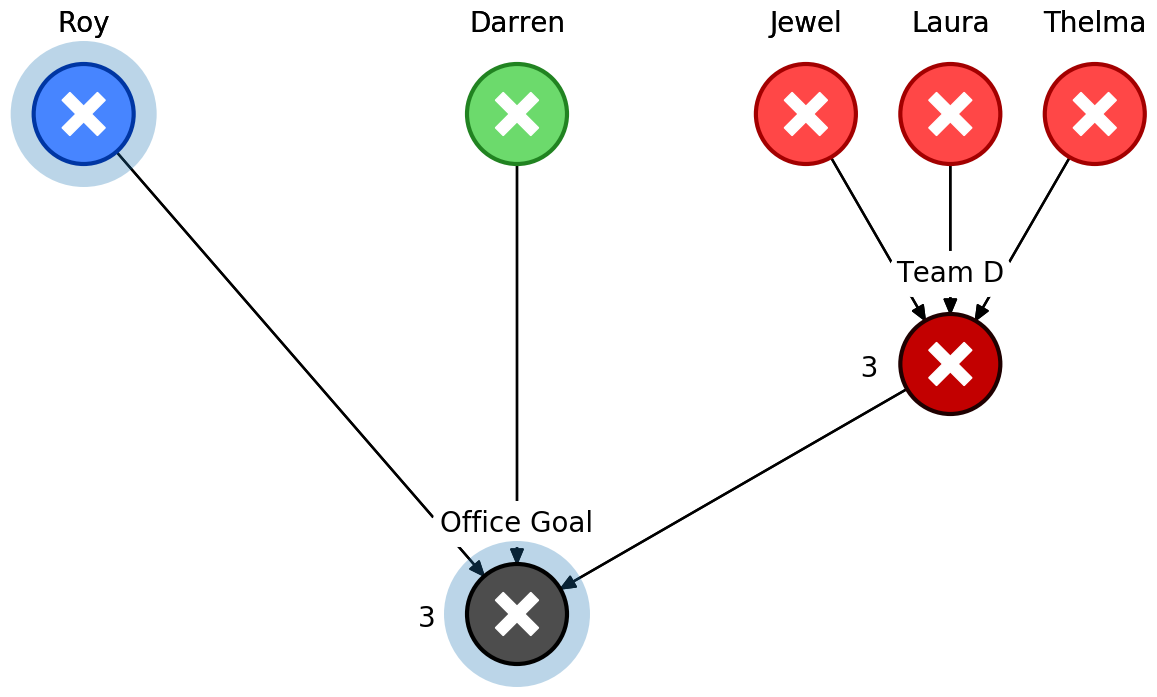
\includegraphics[width=0.22\columnwidth]{situation3}}
{\hfill}
% \caption{caption text}
\end{figure}

\begin{figure}[H]
\renewcommand{\thesubfigure}{\arabic{subfigure}}
\centering
{\hfill}
\subfloat[][]{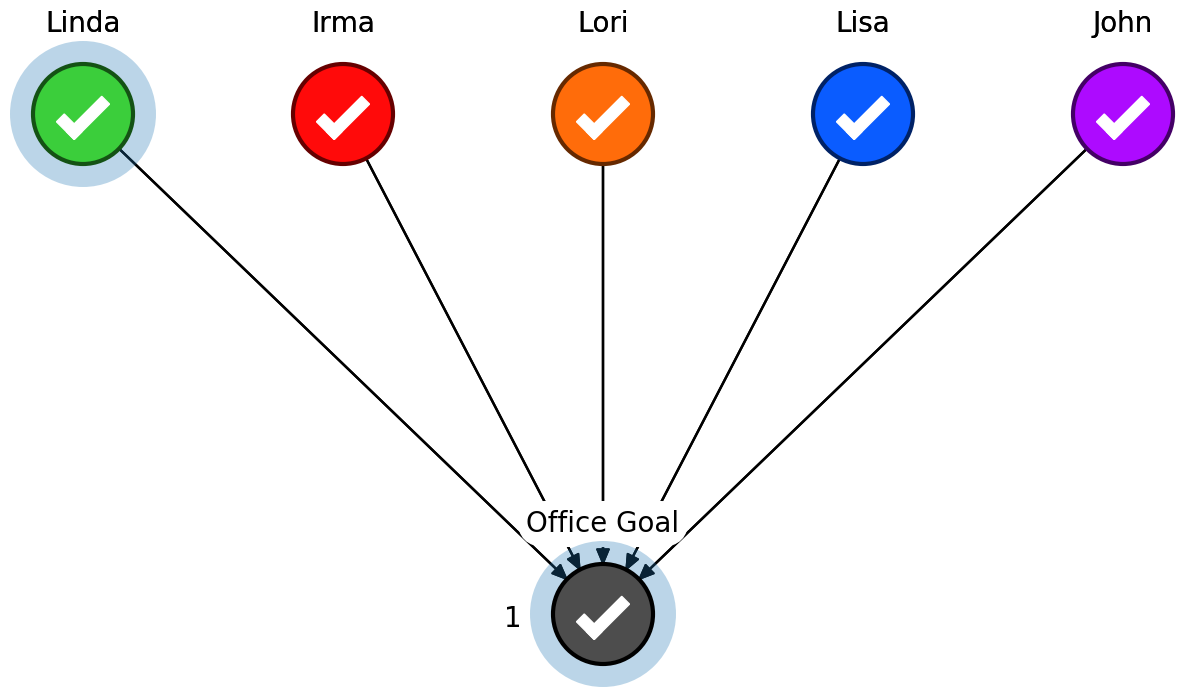
\includegraphics[width=0.22\columnwidth]{situation4}}
\hfill
\subfloat[][]{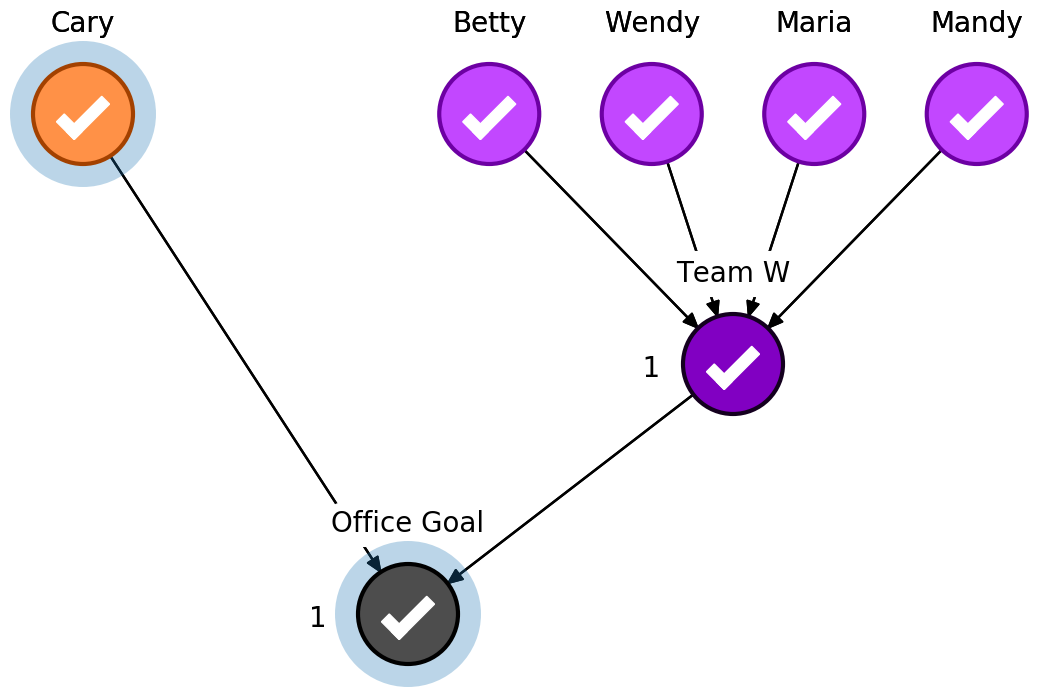
\includegraphics[width=0.22\columnwidth]{situation5}}
\hfill
\subfloat[][]{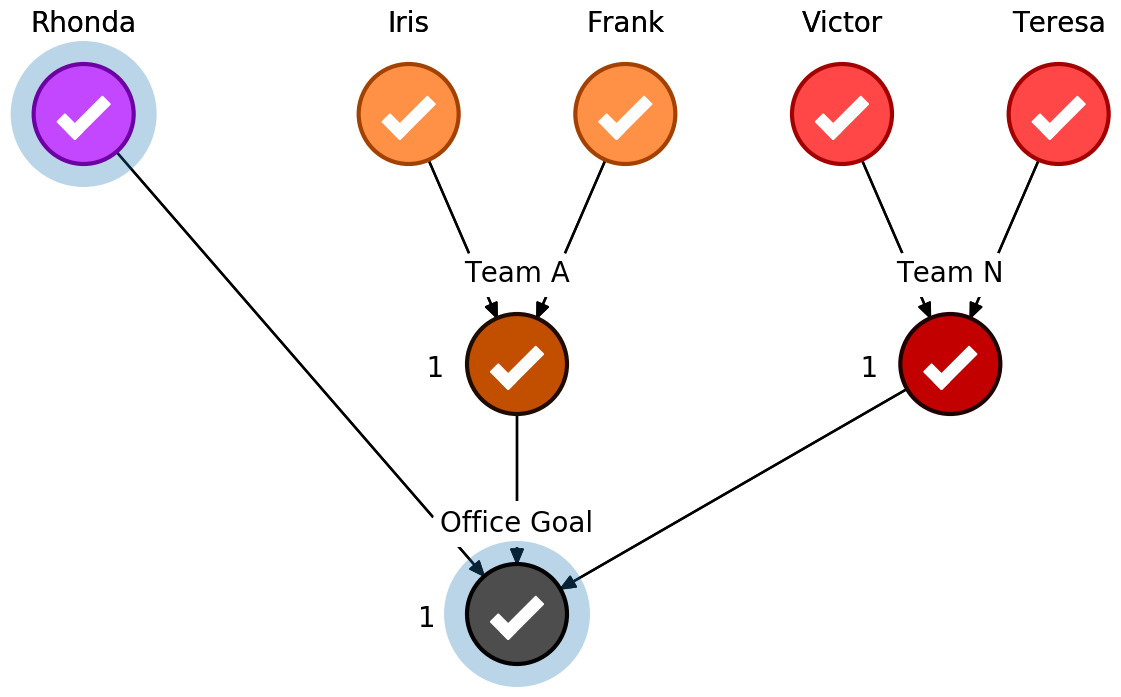
\includegraphics[width=0.22\columnwidth]{situation6}}
\hfill
\subfloat[][]{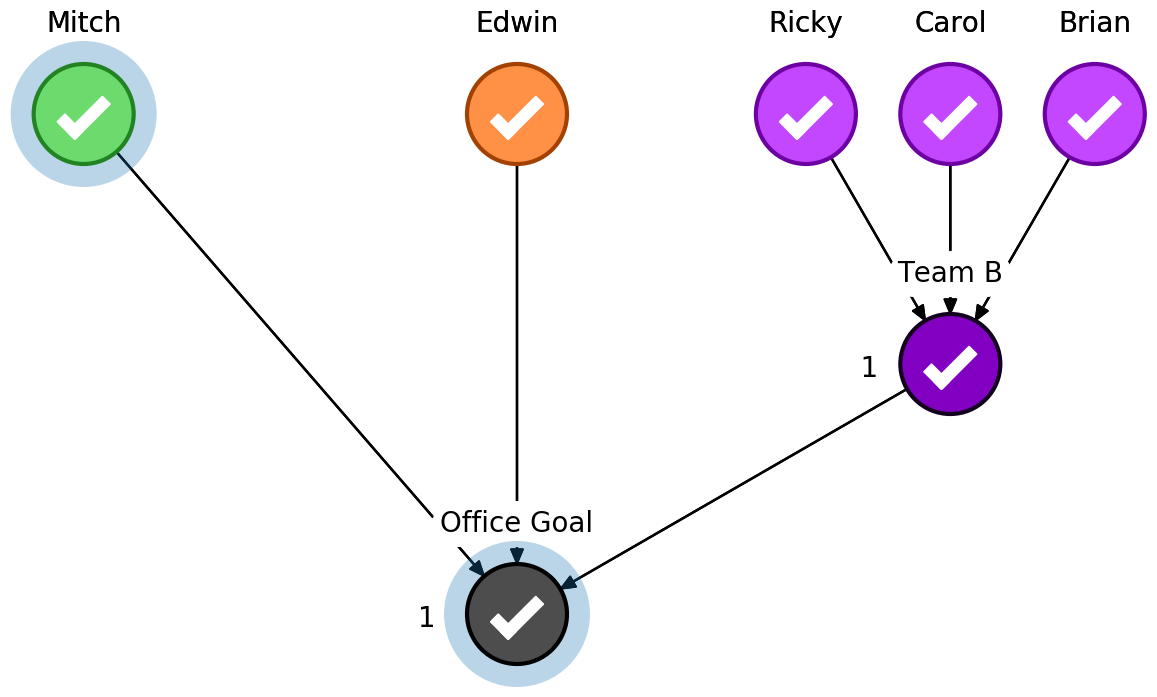
\includegraphics[width=0.22\columnwidth]{situation7}}
{\hfill}
% \caption{caption text}
\end{figure}

\begin{figure}[H]
\renewcommand{\thesubfigure}{\arabic{subfigure}}
\centering
{\hfill}
\subfloat[][]{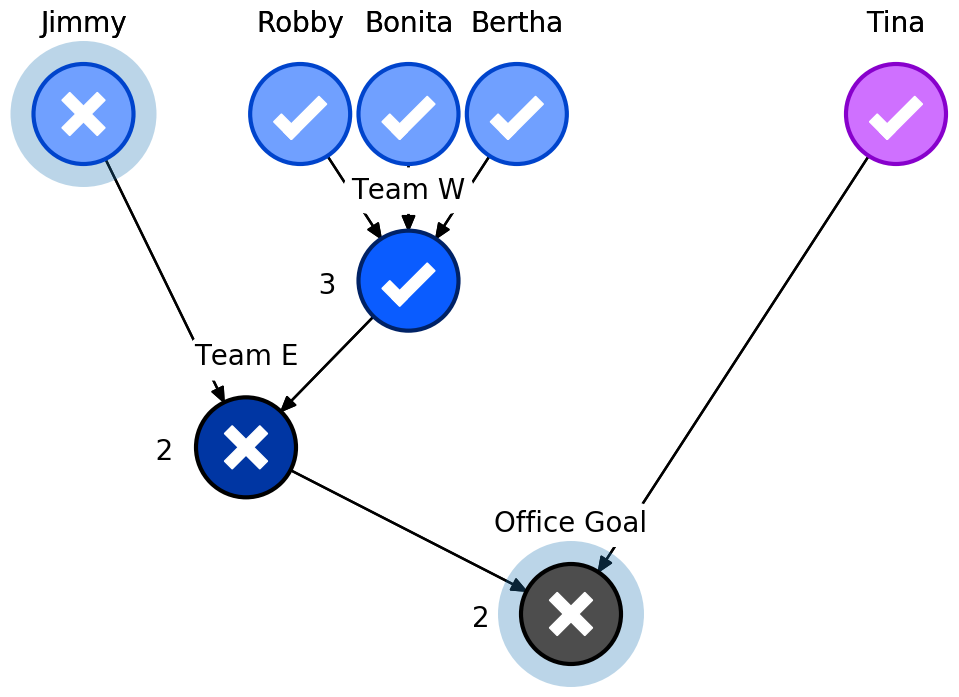
\includegraphics[width=0.22\columnwidth]{situation8}}
\hfill
\subfloat[][]{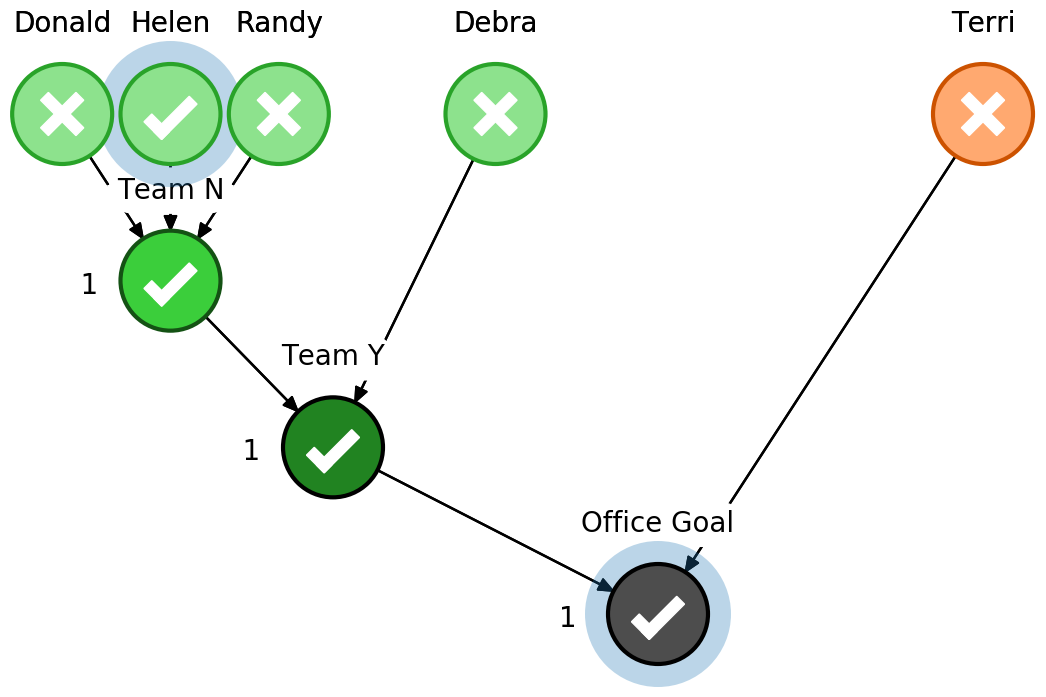
\includegraphics[width=0.22\columnwidth]{situation9}}
\hfill
\subfloat[][]{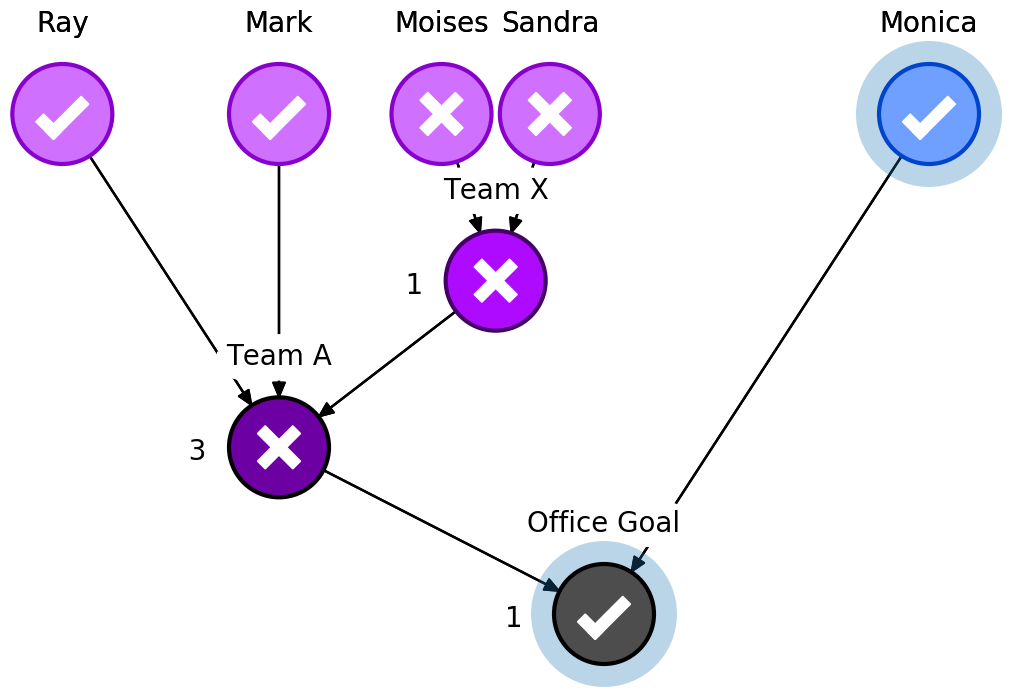
\includegraphics[width=0.22\columnwidth]{situation10}}
\hfill
\subfloat[][]{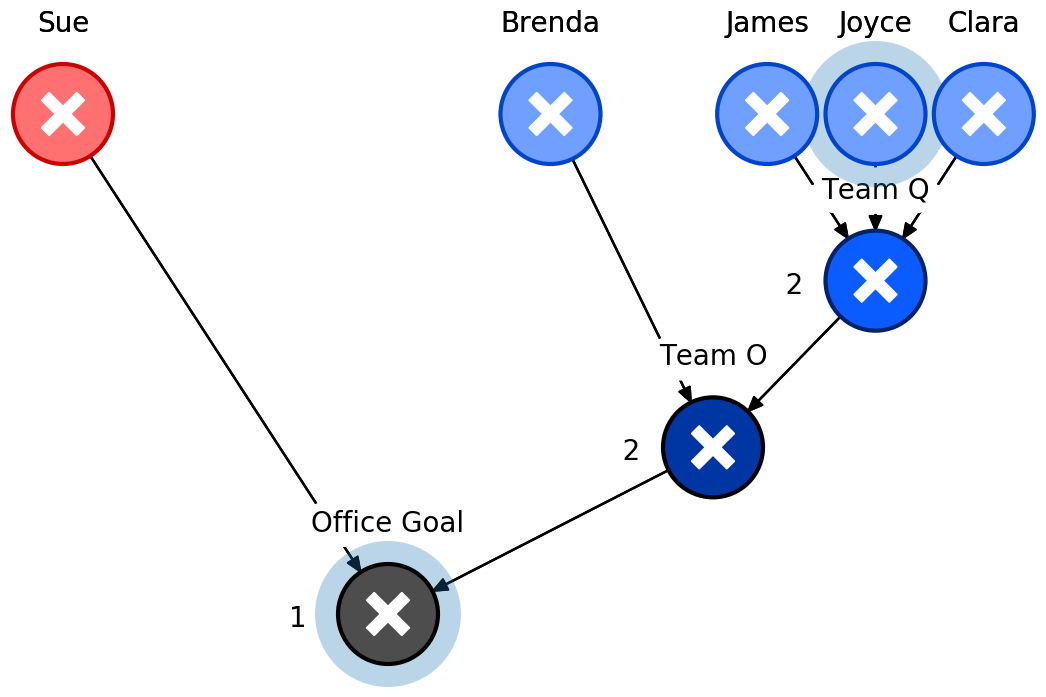
\includegraphics[width=0.22\columnwidth]{situation11}}
{\hfill}
\end{figure}

\begin{figure}[H]
\renewcommand{\thesubfigure}{\arabic{subfigure}}
\centering
{\hfill}
\subfloat[][]{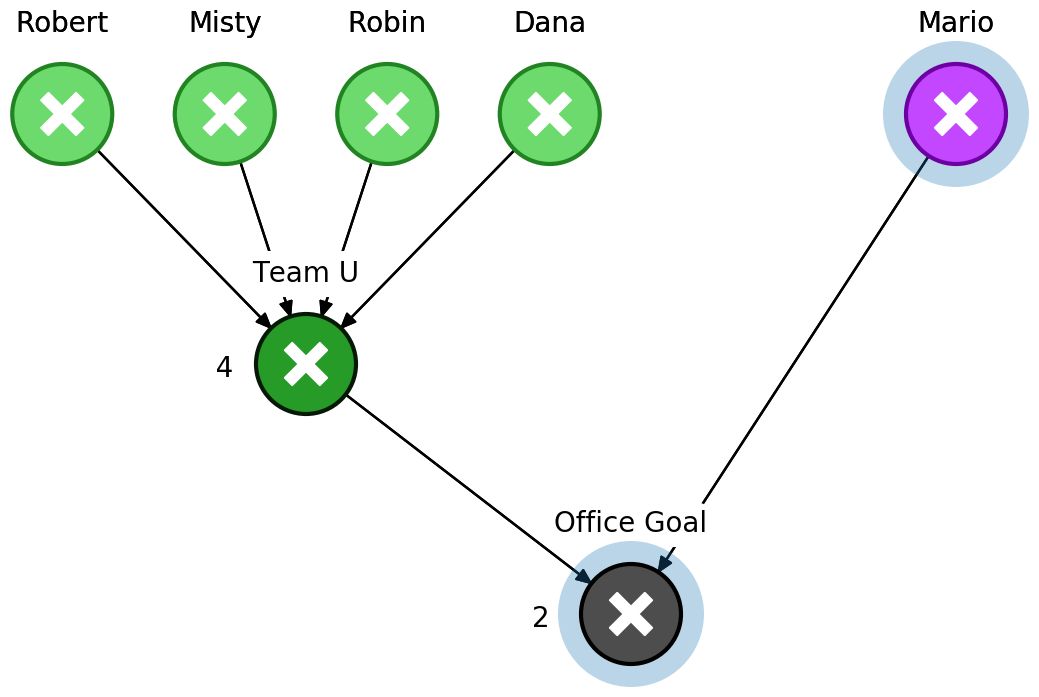
\includegraphics[width=0.22\columnwidth]{situation12}}
\hfill
\subfloat[][]{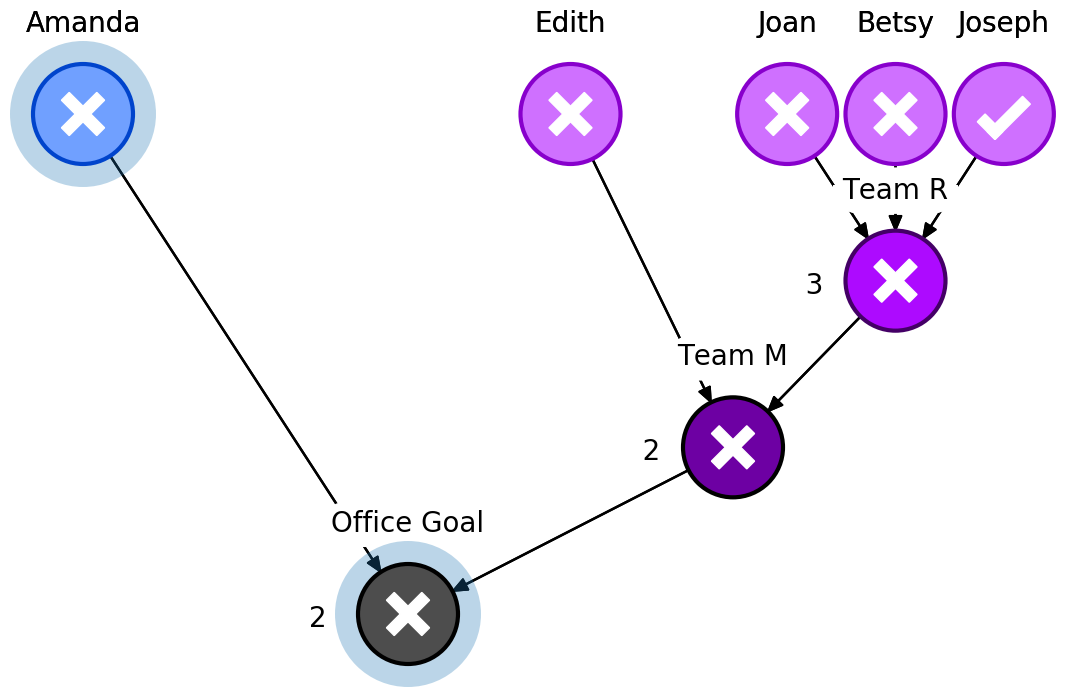
\includegraphics[width=0.22\columnwidth]{situation13}}
\hfill
\subfloat[][]{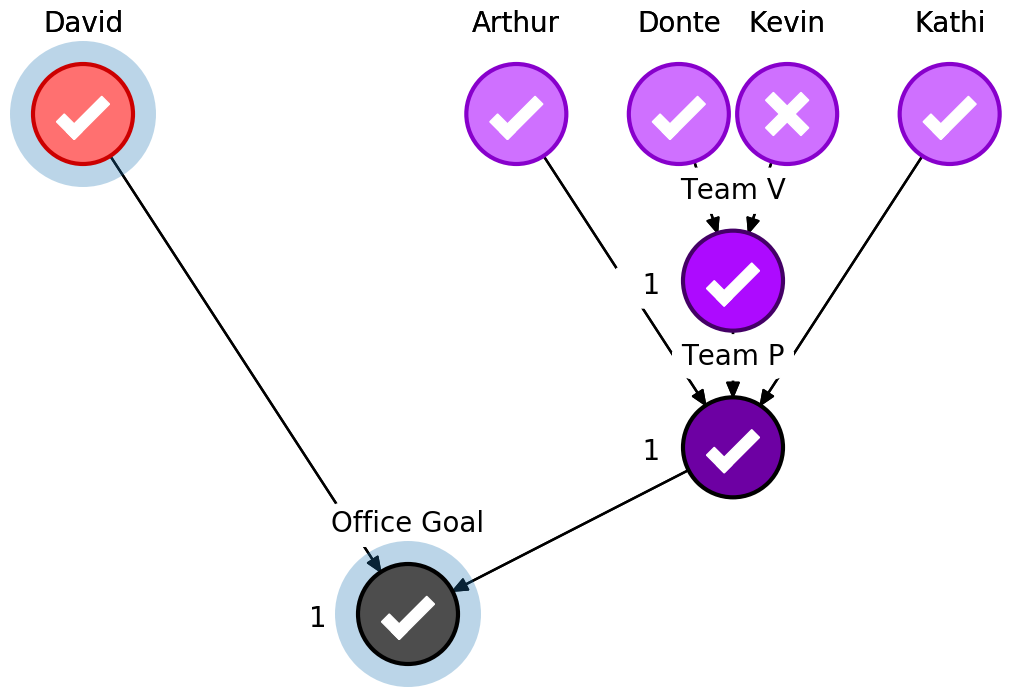
\includegraphics[width=0.22\columnwidth]{situation14}}
\hfill
\subfloat[][]{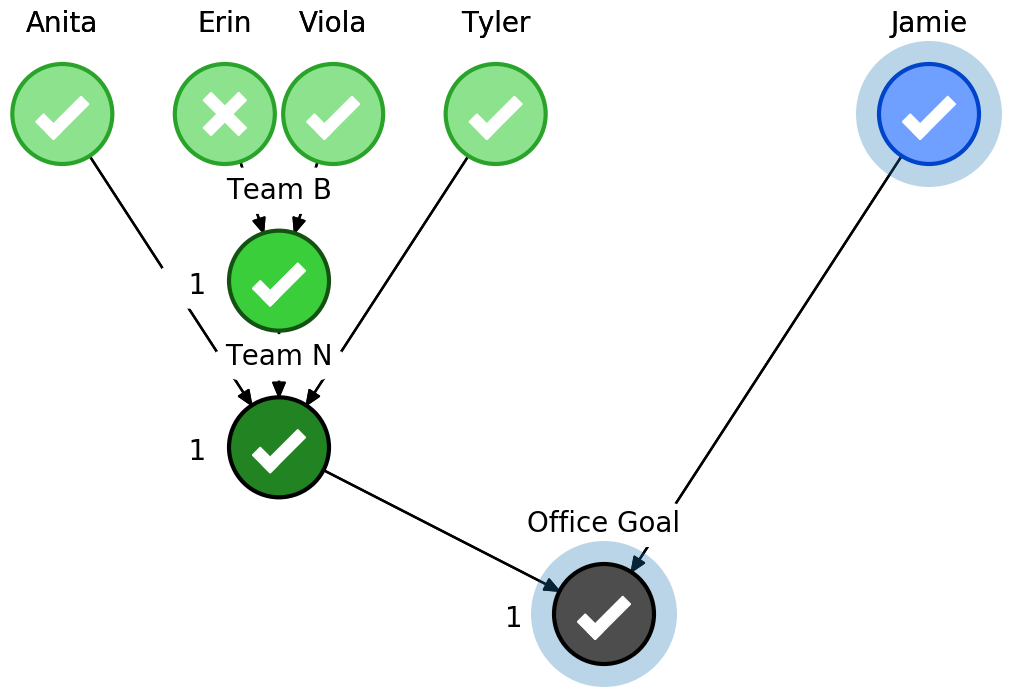
\includegraphics[width=0.22\columnwidth]{situation15}}
{\hfill}
\caption{16 Different situations used in Experiment 1.}
\end{figure}

\subsubsection{Procedure}
\label{ssub:procedure}

\begin{figure}[H]
	\centering
	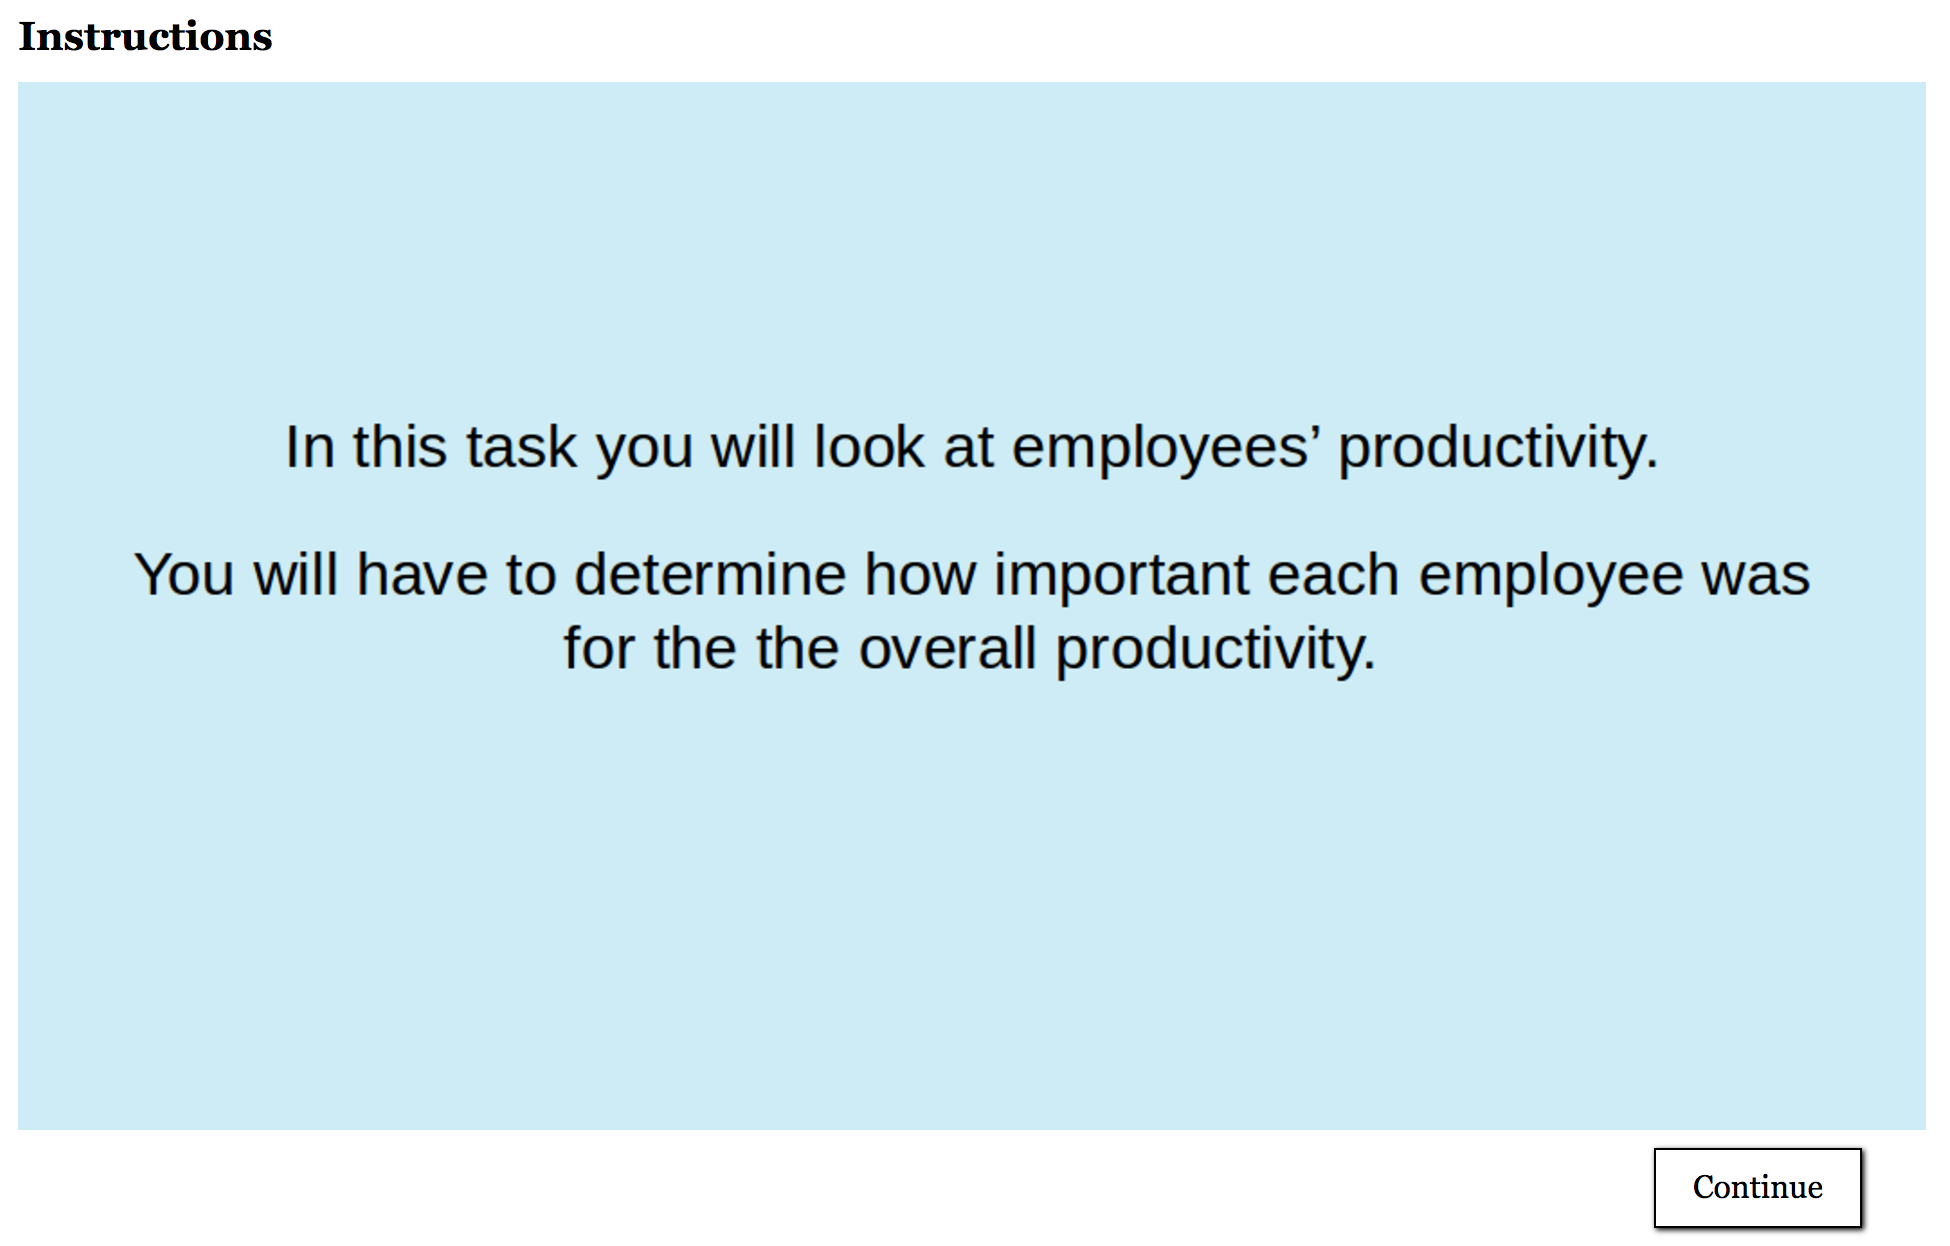
\includegraphics[width=0.95\textwidth]{screenshot_1}
	\caption{Instruction screenshot 1.}
	\label{fig:screenshot_1}
\end{figure}
\begin{figure}[H]
	\centering
	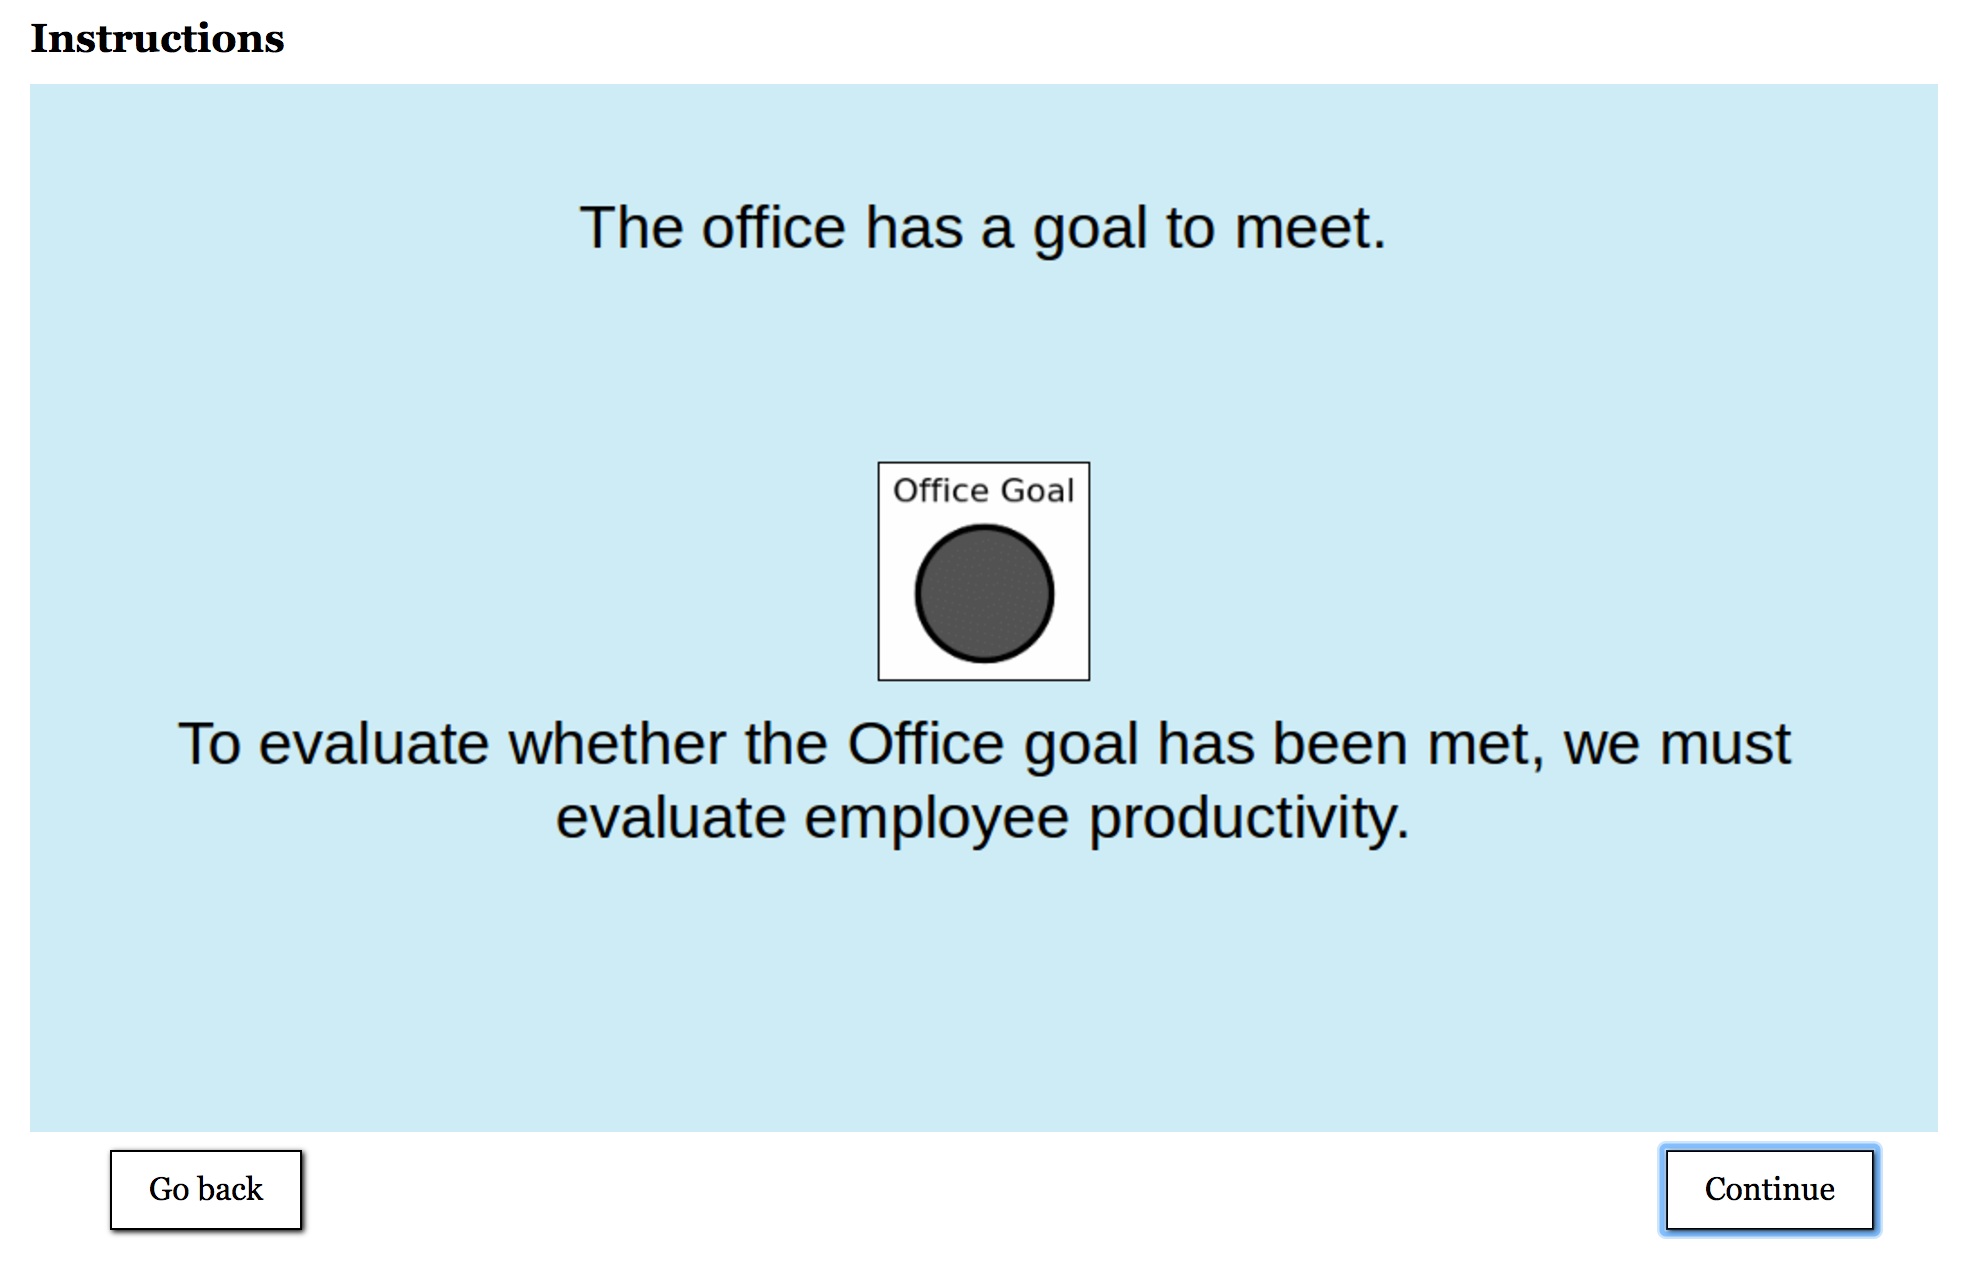
\includegraphics[width=0.95\textwidth]{screenshot_2}
	\caption{Instruction screenshot 2.}
	\label{fig:screenshot_2}
\end{figure}
\begin{figure}[H]
	\centering
	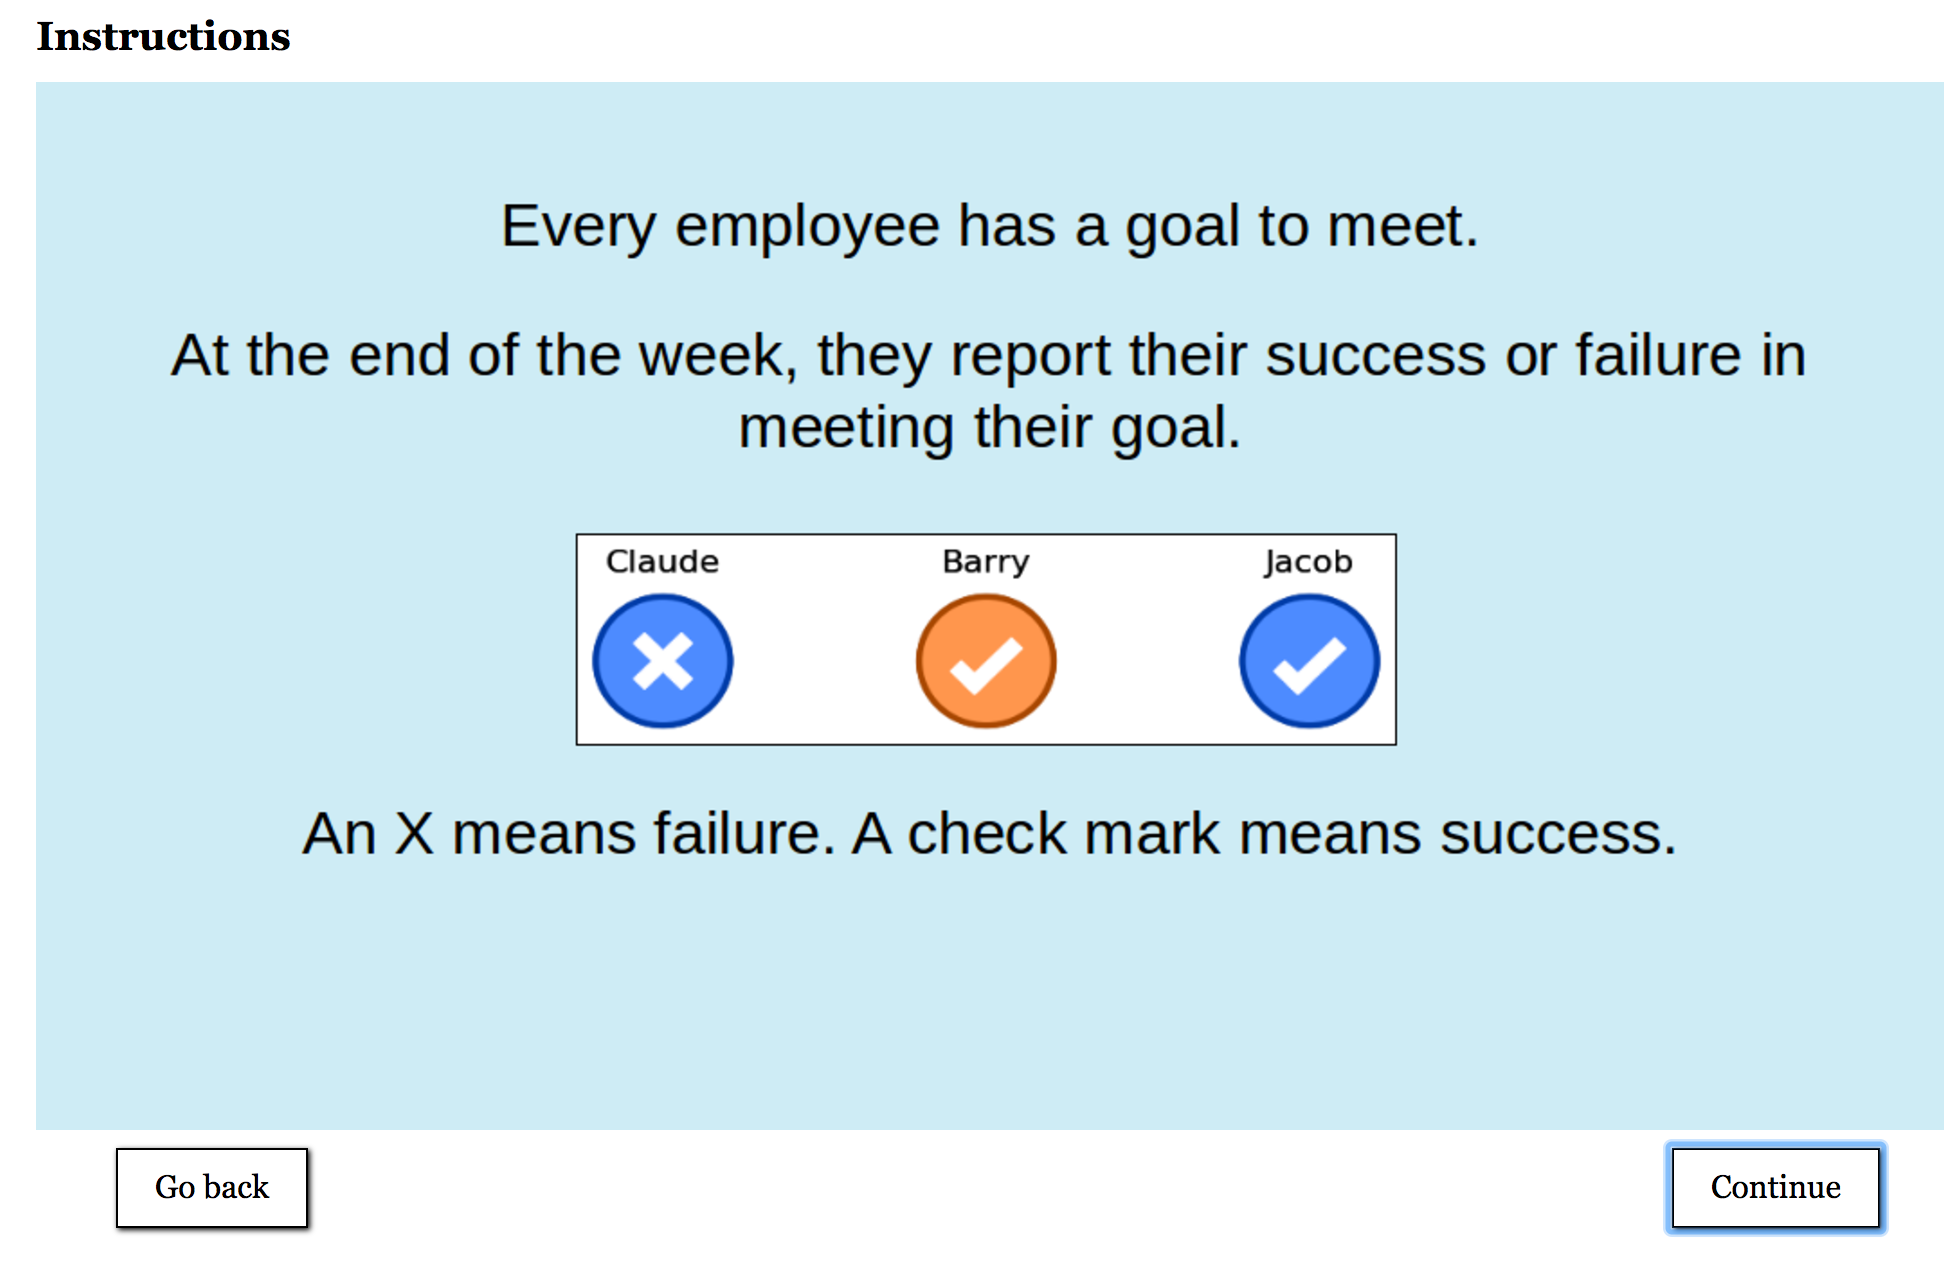
\includegraphics[width=0.95\textwidth]{screenshot_3}
	\caption{Instruction screenshot 3.}
	\label{fig:screenshot_3}
\end{figure}
\begin{figure}[H]
	\centering
	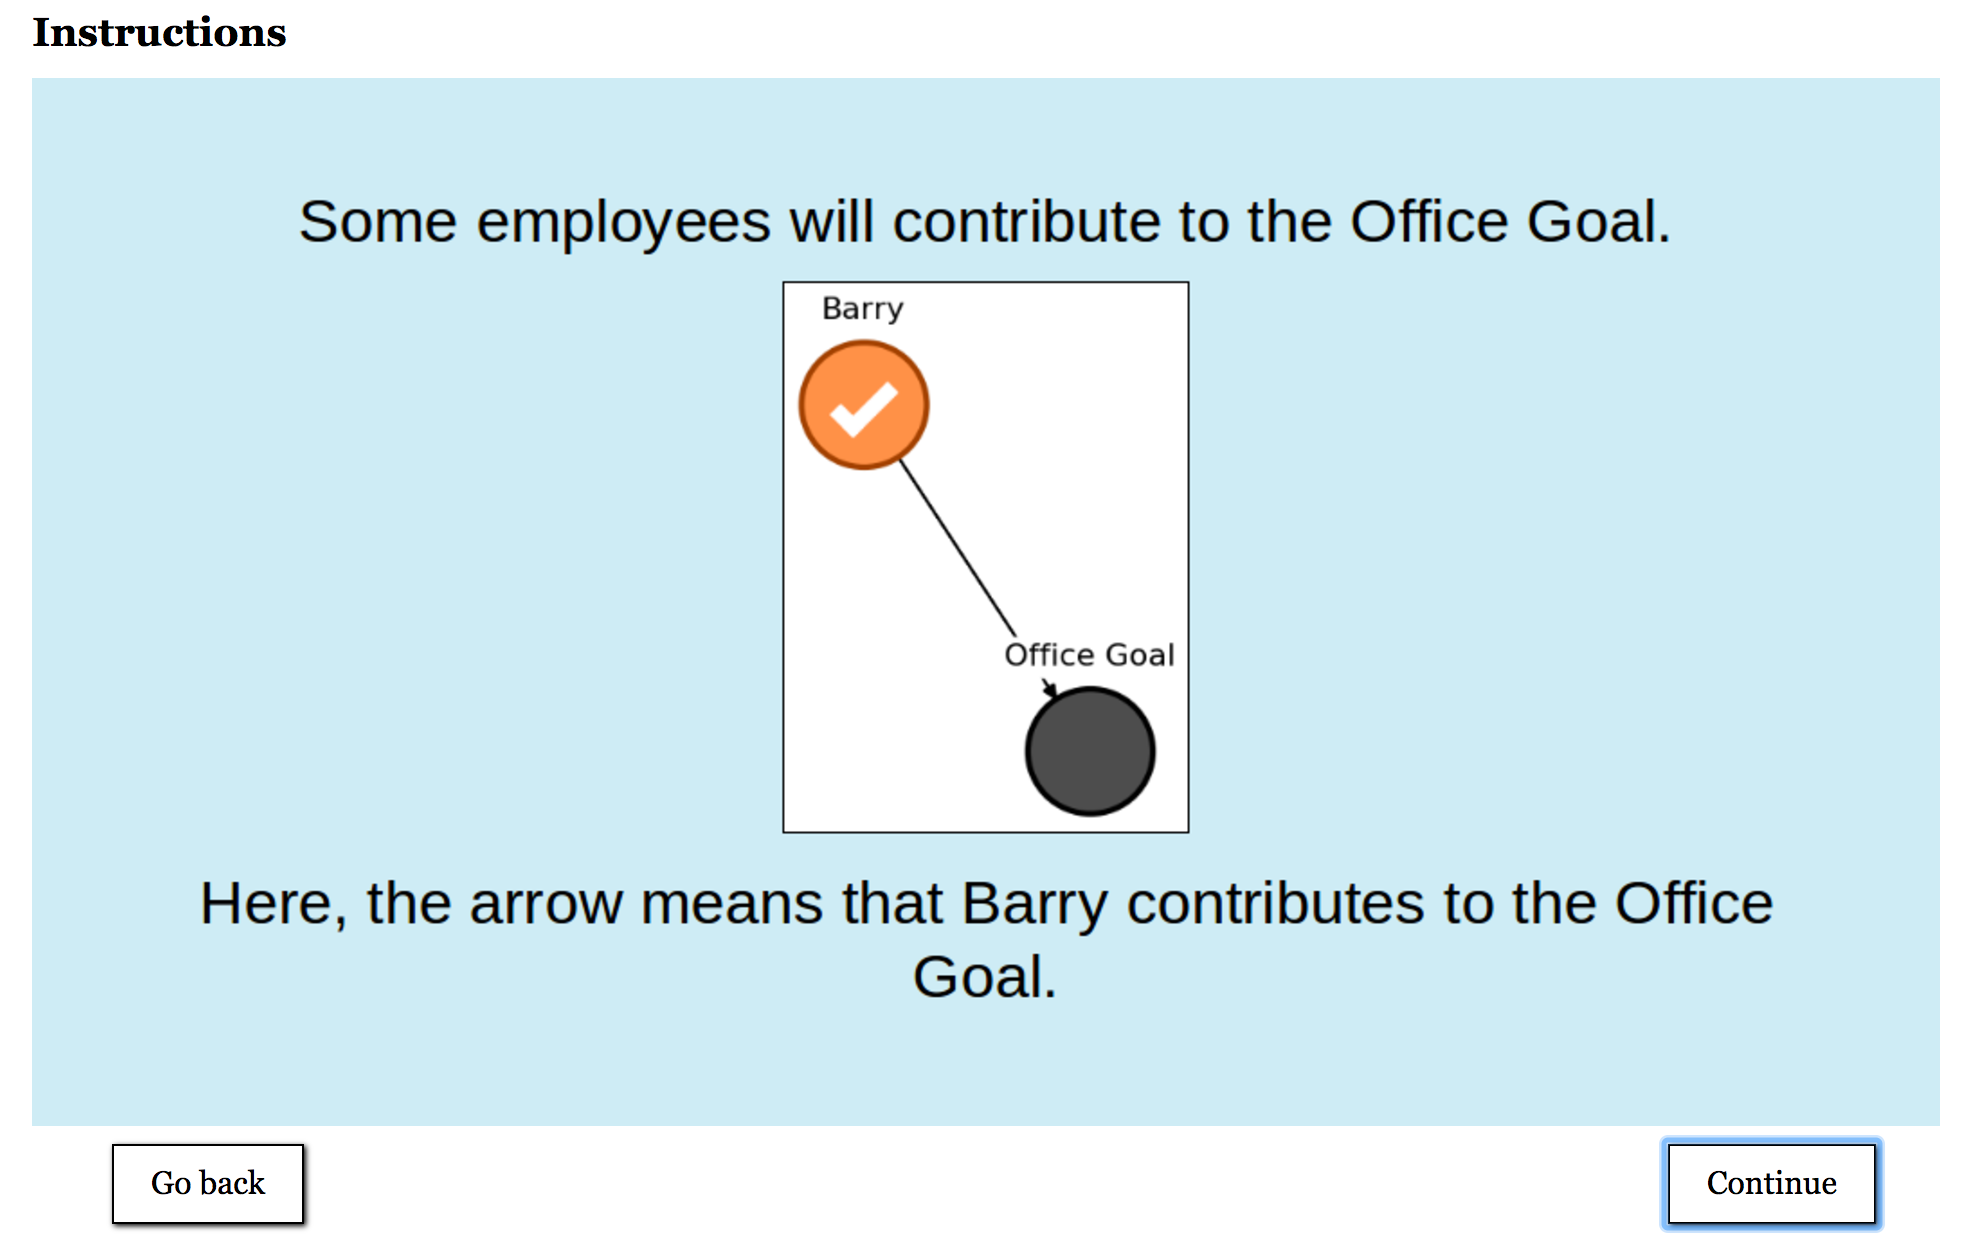
\includegraphics[width=0.95\textwidth]{screenshot_4}
	\caption{Instruction screenshot 4.}
	\label{fig:screenshot_4}
\end{figure}
\begin{figure}[H]
	\centering
	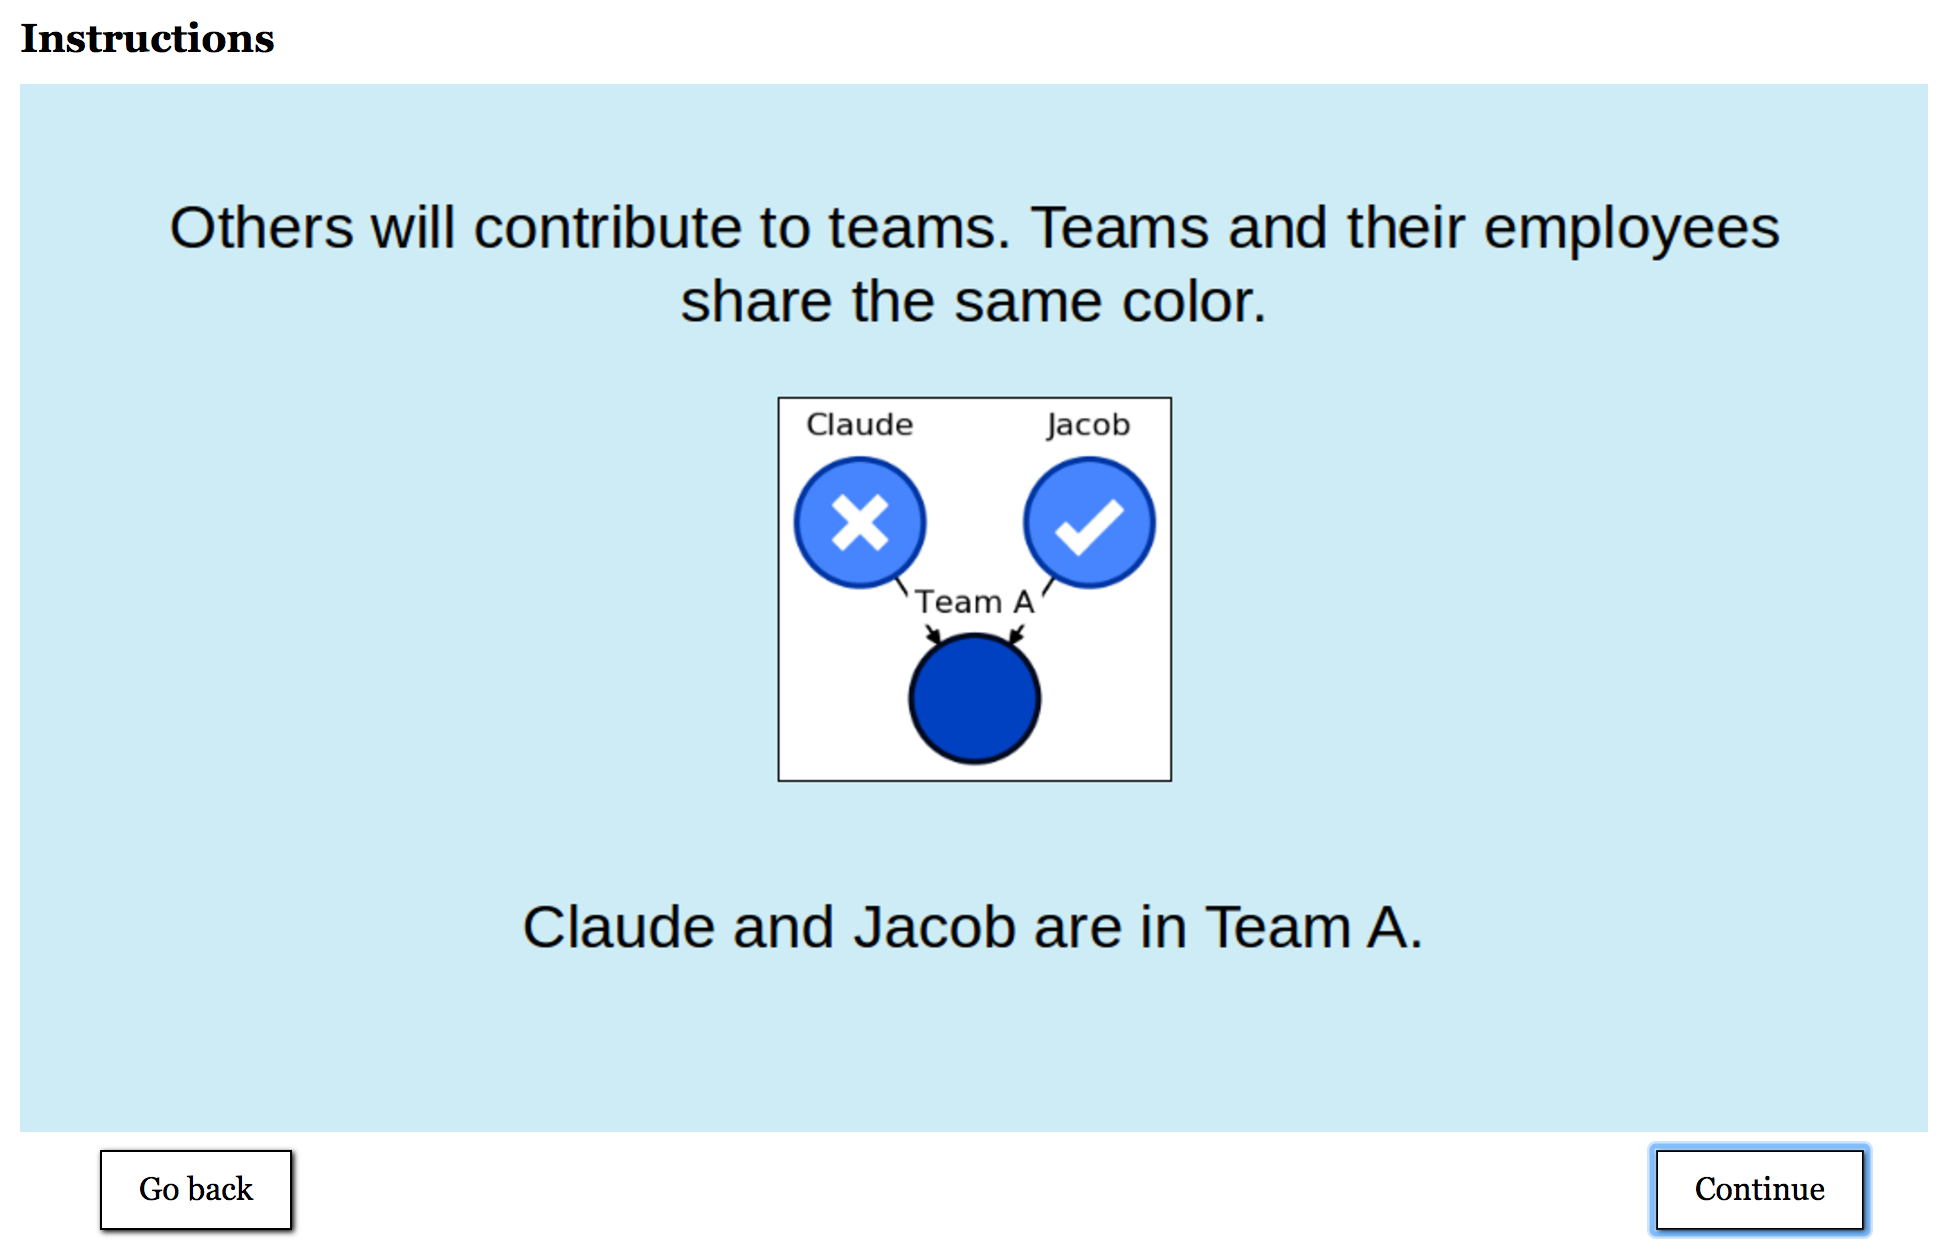
\includegraphics[width=0.95\textwidth]{screenshot_5}
	\caption{Instruction screenshot 5.}
	\label{fig:screenshot_5}
\end{figure}
\begin{figure}[H]
	\centering
	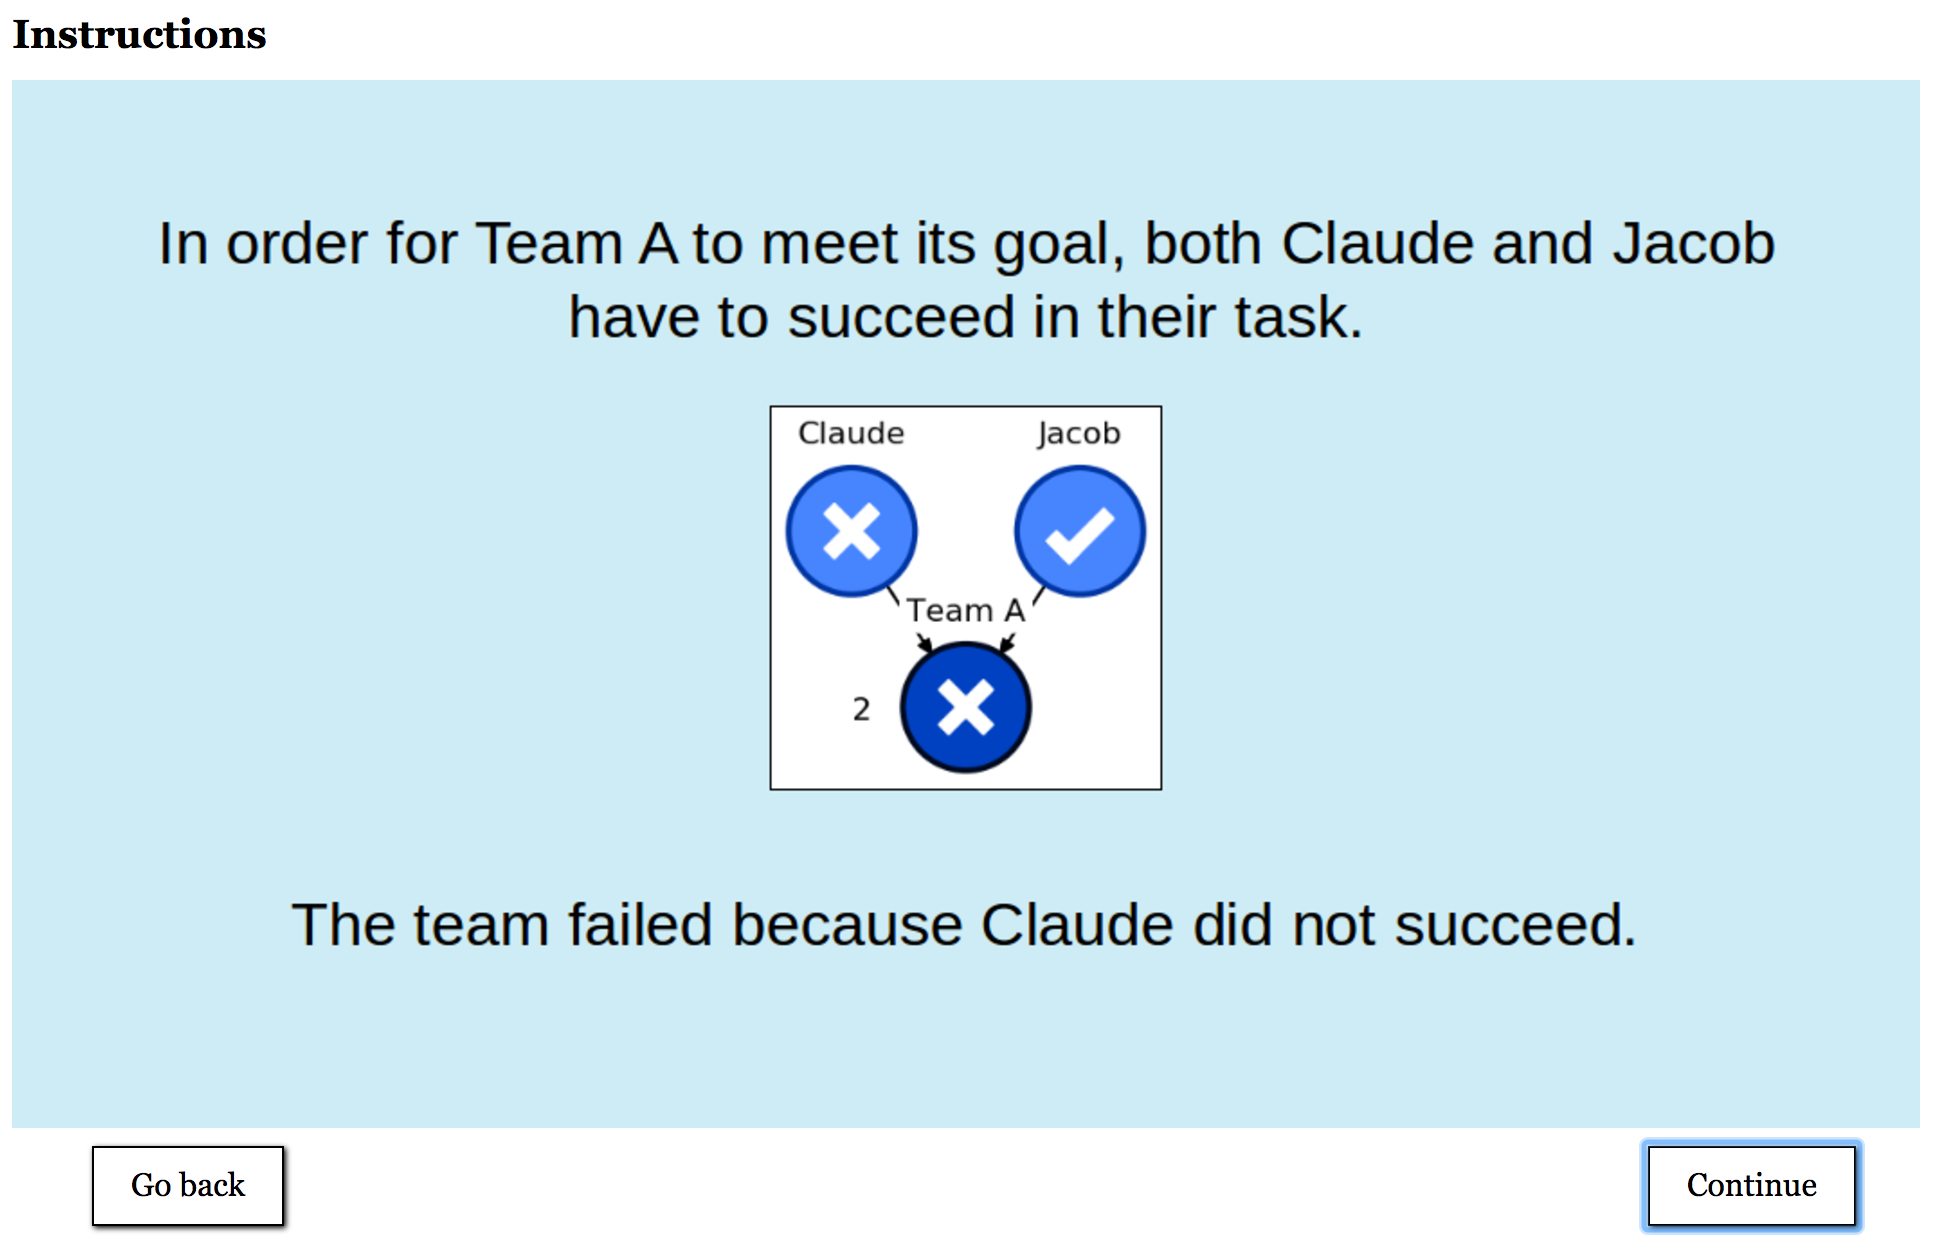
\includegraphics[width=0.95\textwidth]{screenshot_6}
	\caption{Instruction screenshot 6.}
	\label{fig:screenshot_6}
\end{figure}
\begin{figure}[H]
	\centering
	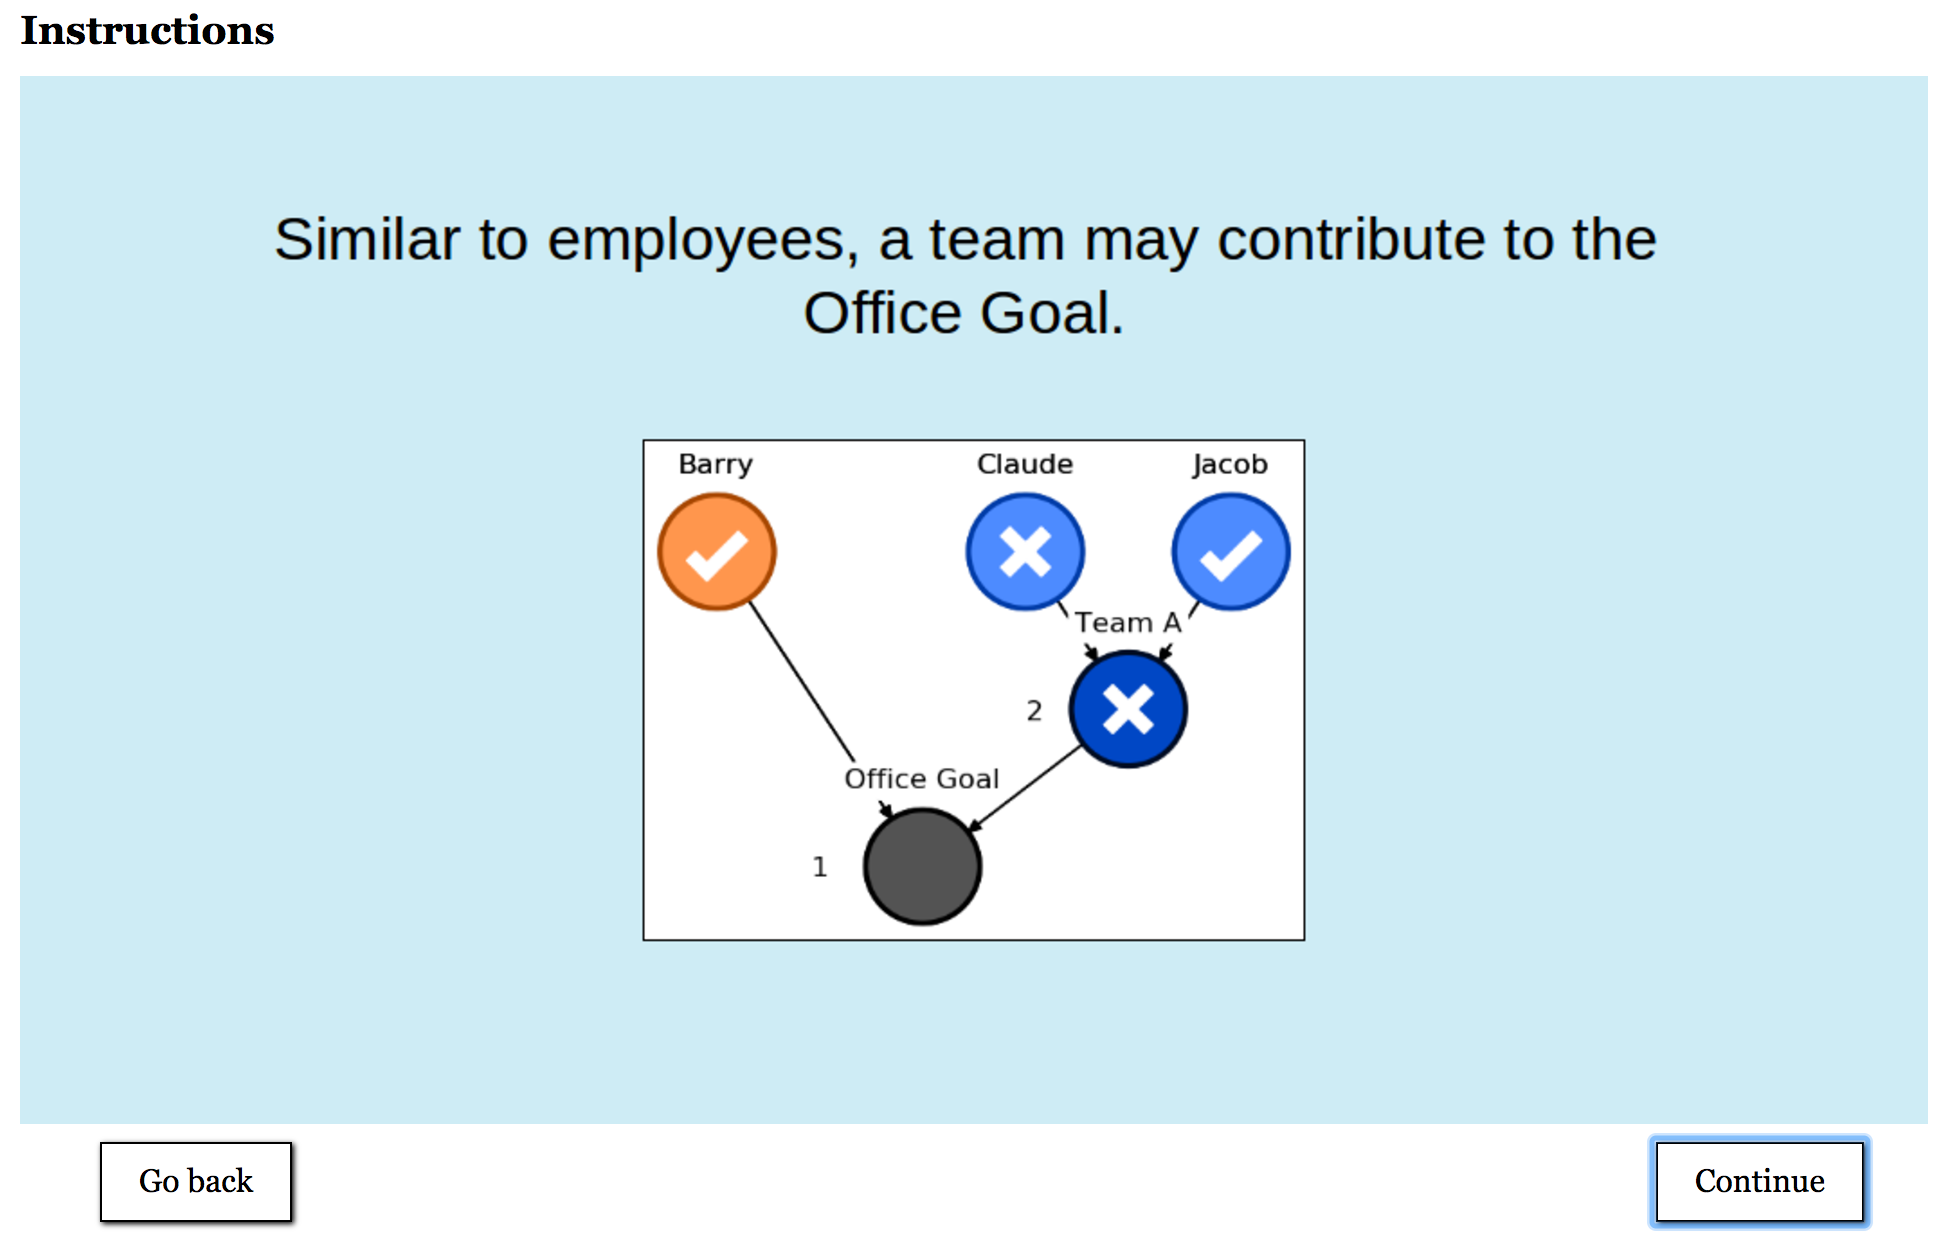
\includegraphics[width=0.95\textwidth]{screenshot_7}
	\caption{Instruction screenshot 7.}
	\label{fig:screenshot_7}
\end{figure}
\begin{figure}[H]
	\centering
	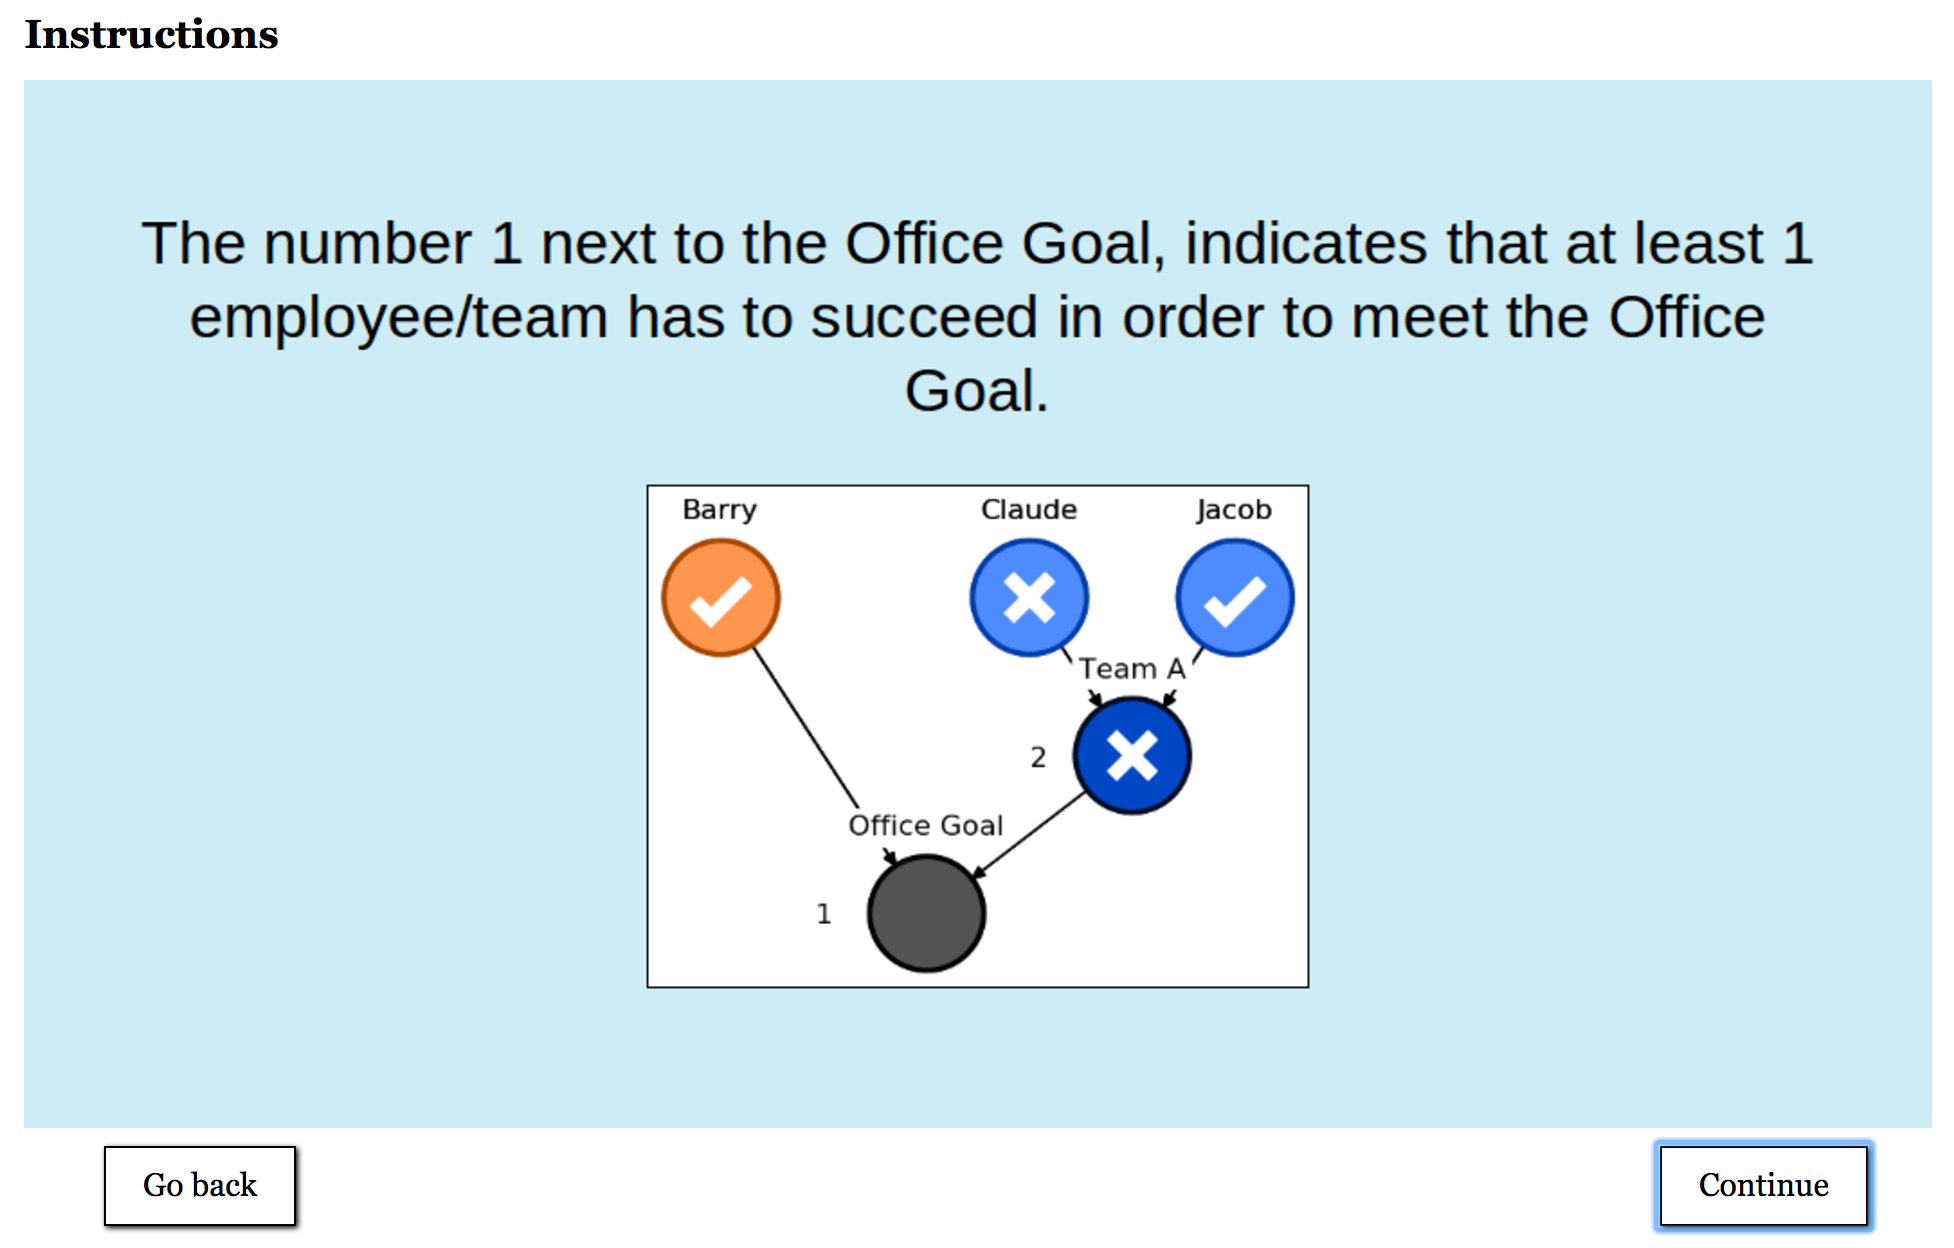
\includegraphics[width=0.95\textwidth]{screenshot_8}
	\caption{Instruction screenshot 8.}
	\label{fig:screenshot_8}
\end{figure}
\begin{figure}[H]
	\centering
	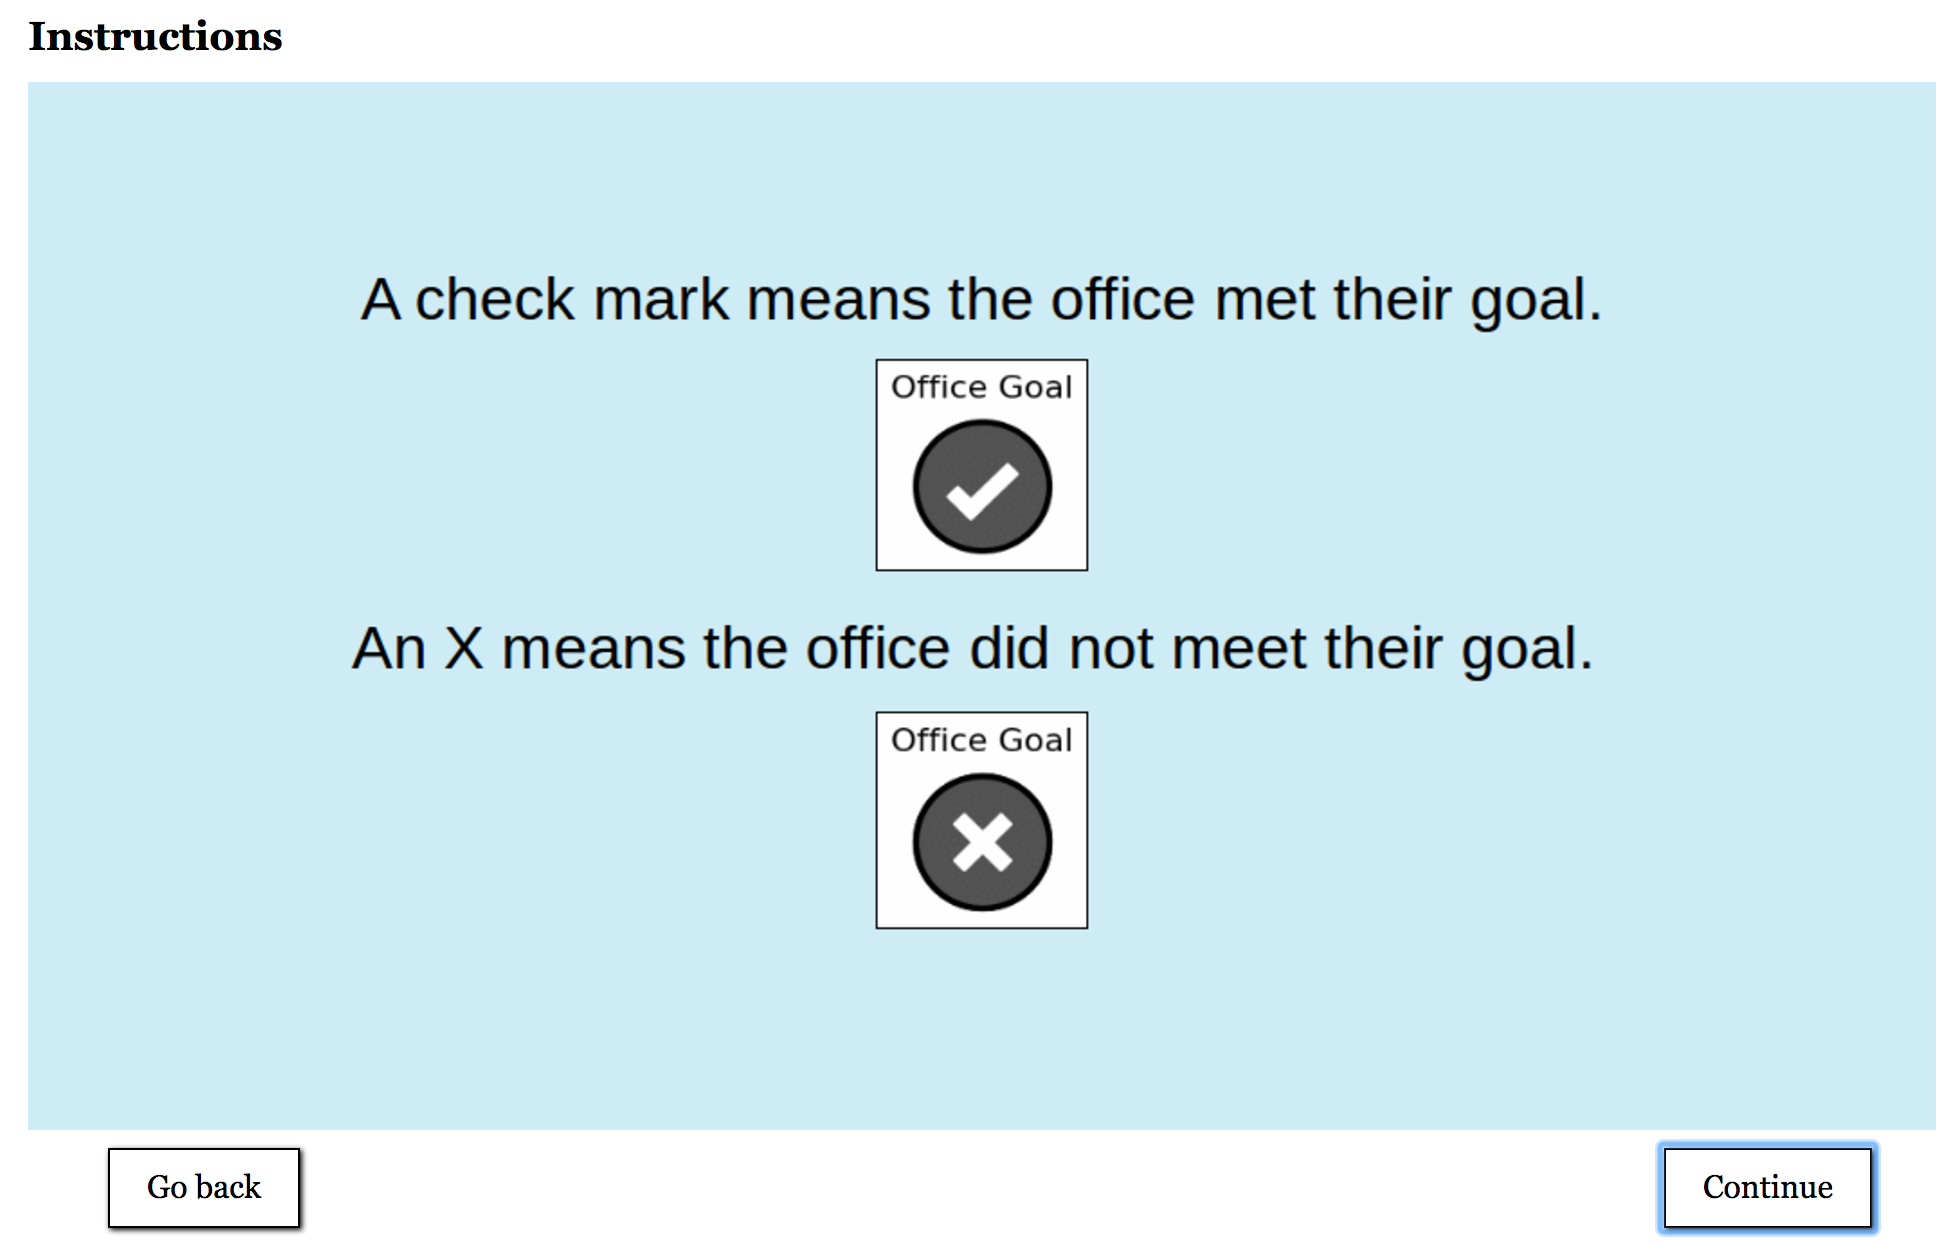
\includegraphics[width=0.95\textwidth]{screenshot_9}
	\caption{Instruction screenshot 9.}
	\label{fig:screenshot_9}
\end{figure}
\begin{figure}[H]
	\centering
	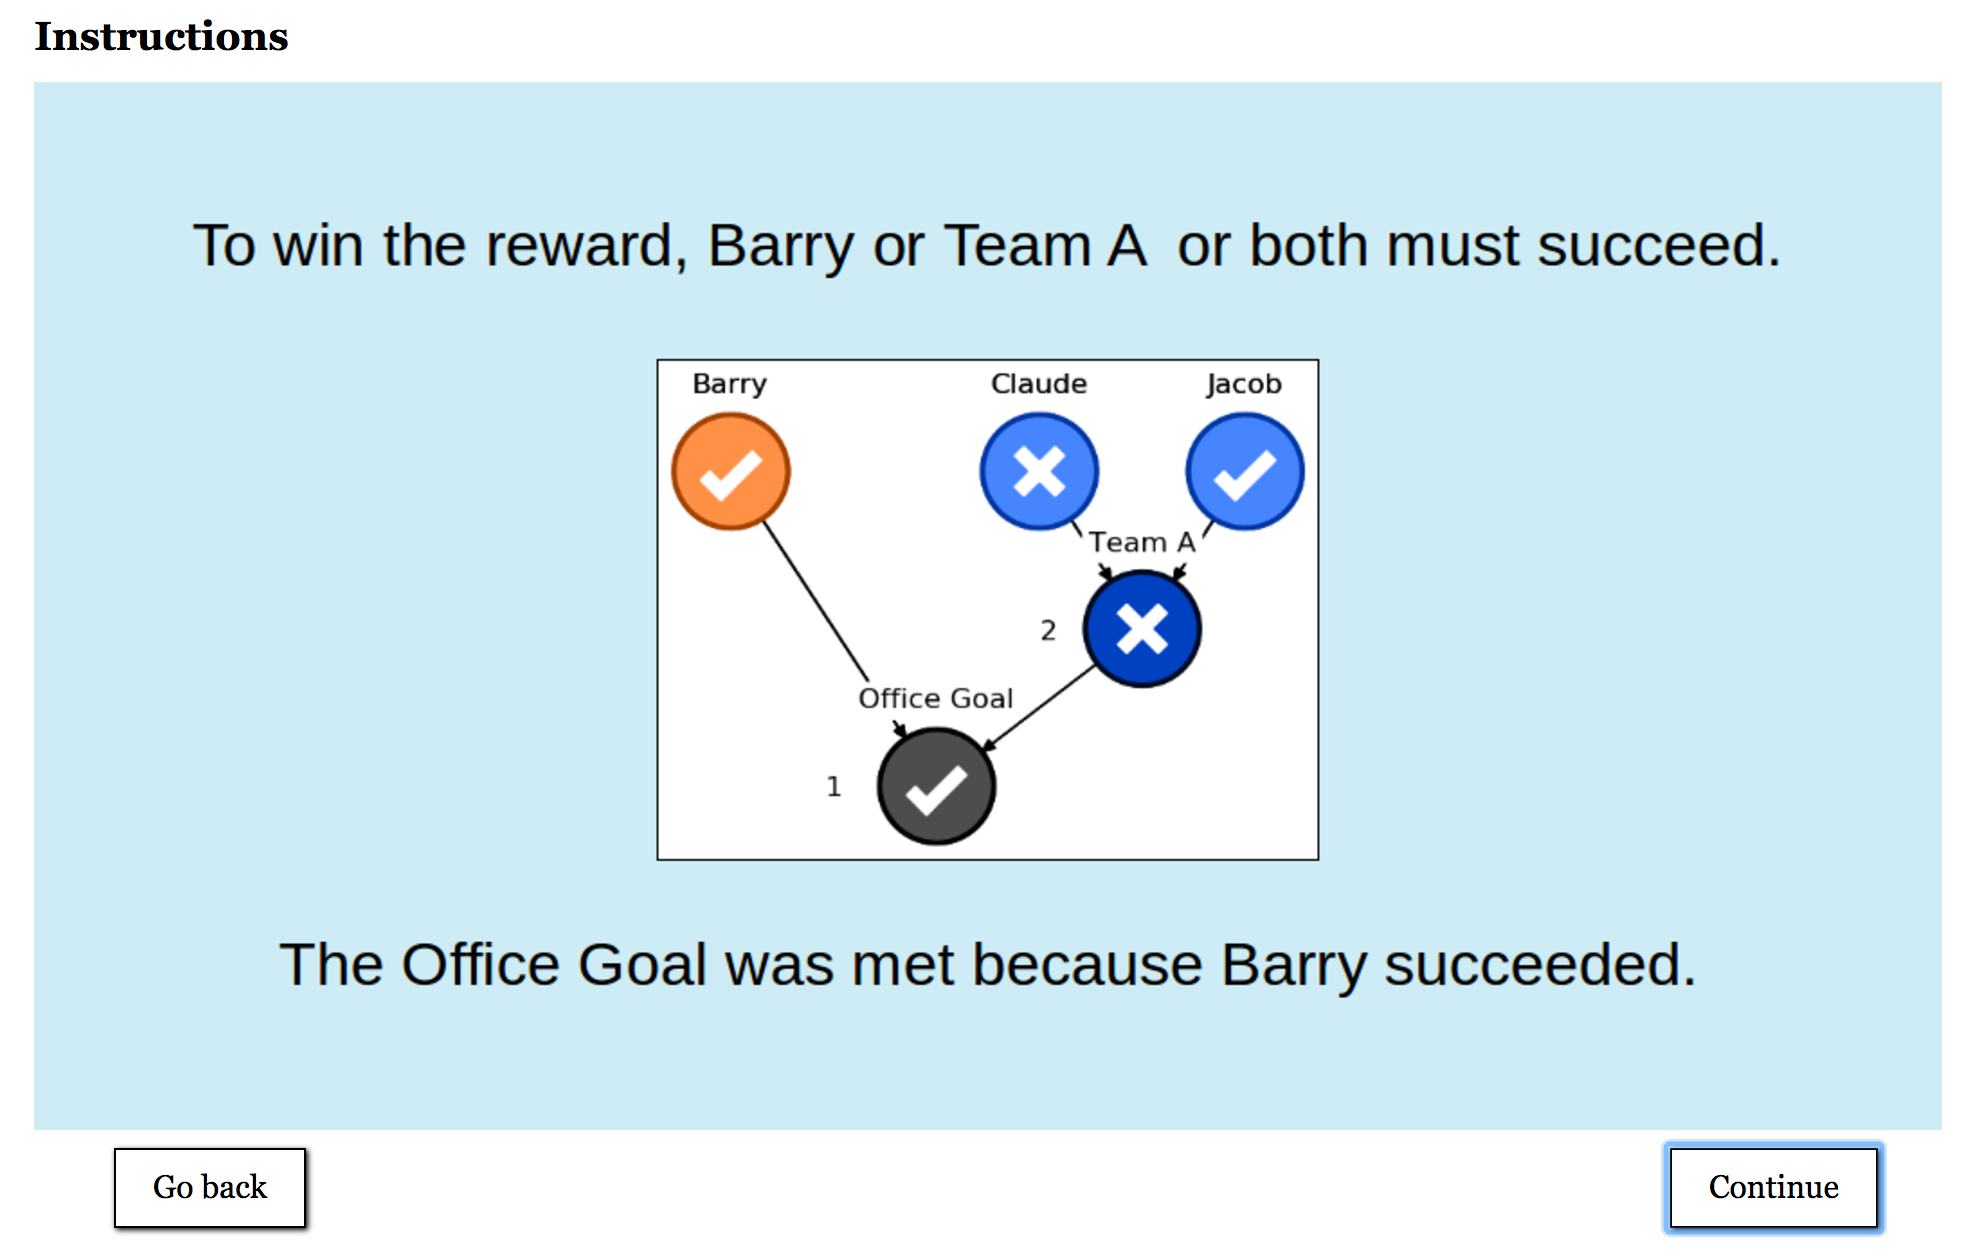
\includegraphics[width=0.95\textwidth]{screenshot_10}
	\caption{Instruction screenshot 10.}
	\label{fig:screenshot_10}
\end{figure}
\begin{figure}[H]
	\centering
	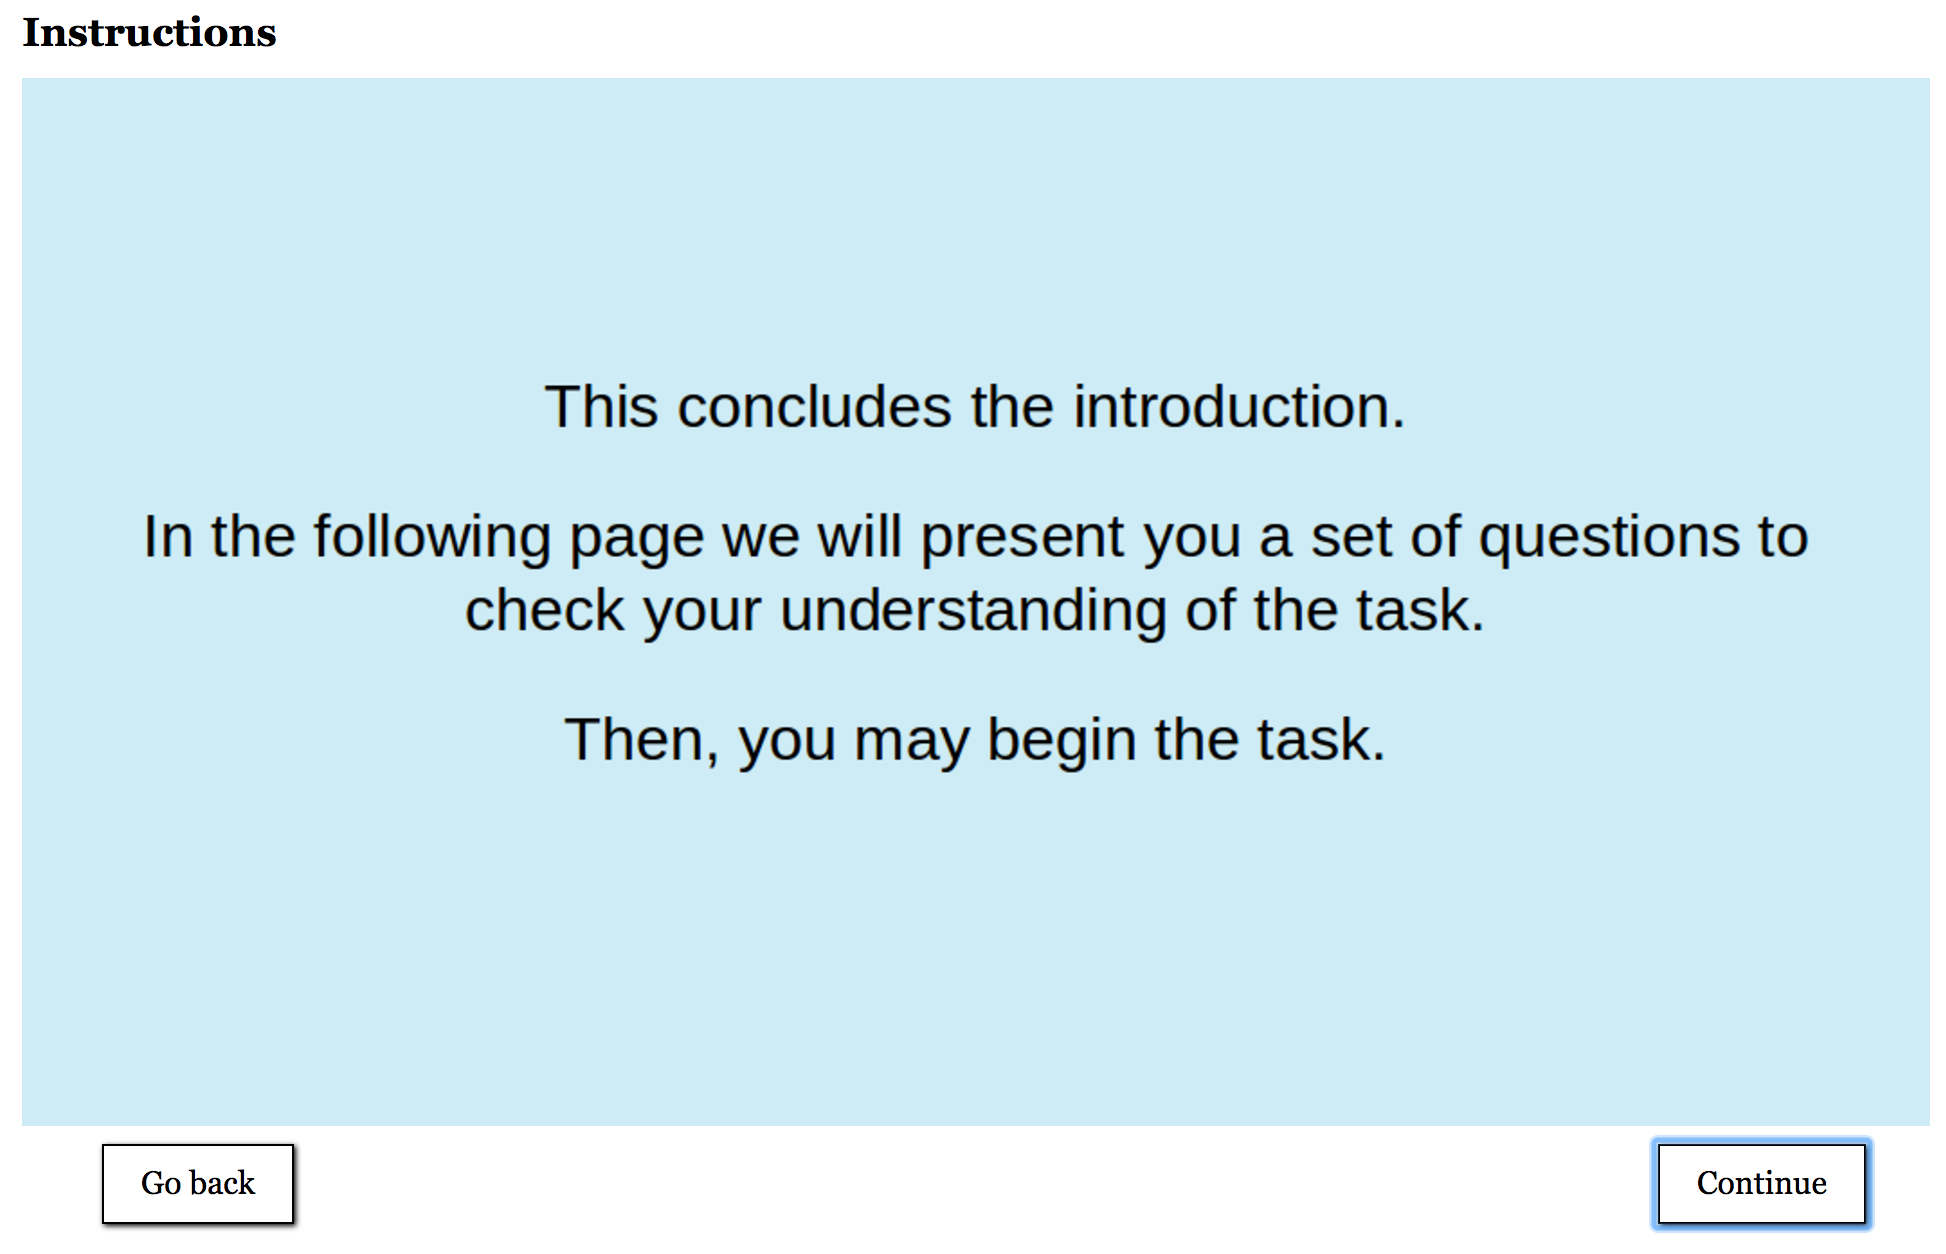
\includegraphics[width=0.95\textwidth]{screenshot_11}
	\caption{Instruction screenshot 11.}
	\label{fig:screenshot_11}
\end{figure}
\begin{figure}[H]
	\centering
	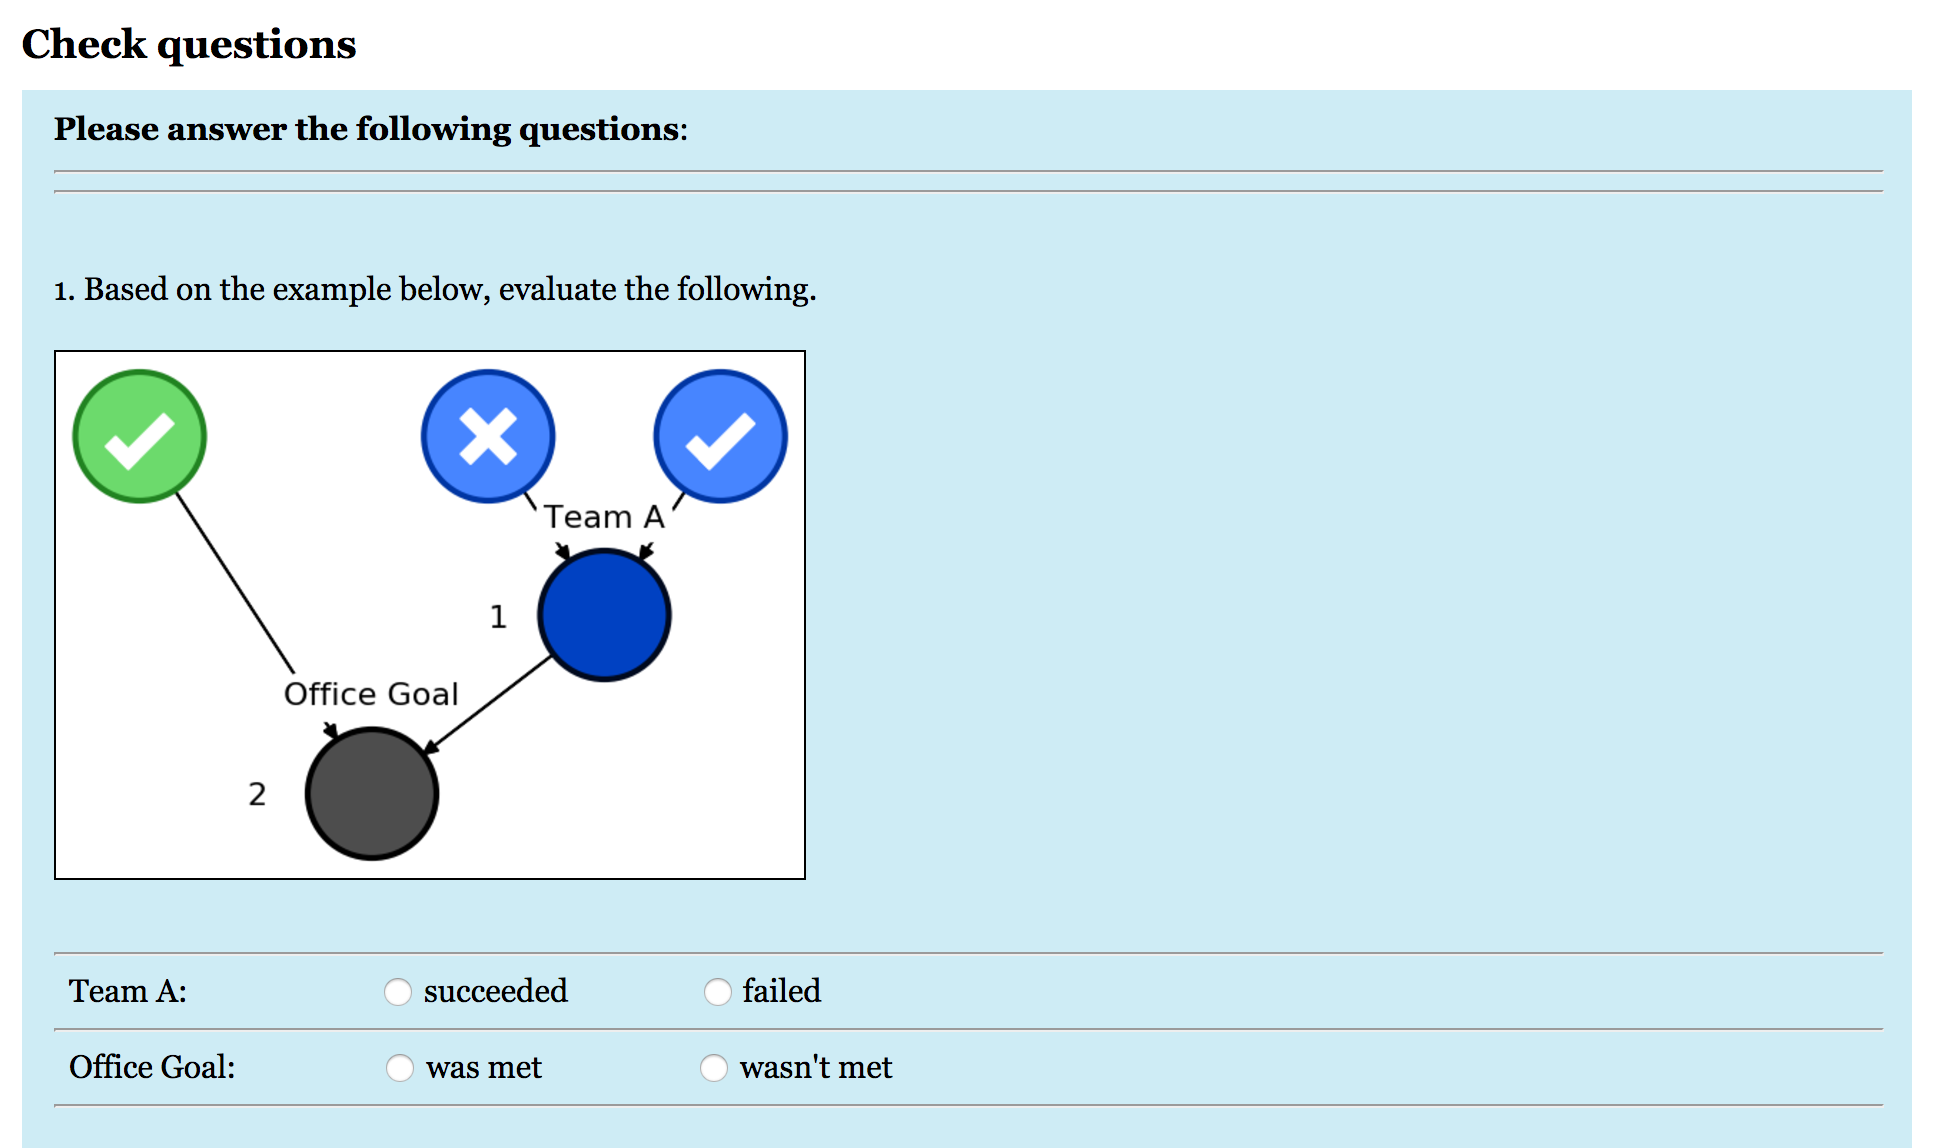
\includegraphics[width=0.95\textwidth]{screenshot_12}
	\caption{Instruction screenshot 12.}
	\label{fig:screenshot_12}
\end{figure}
\begin{figure}[H]
	\centering
	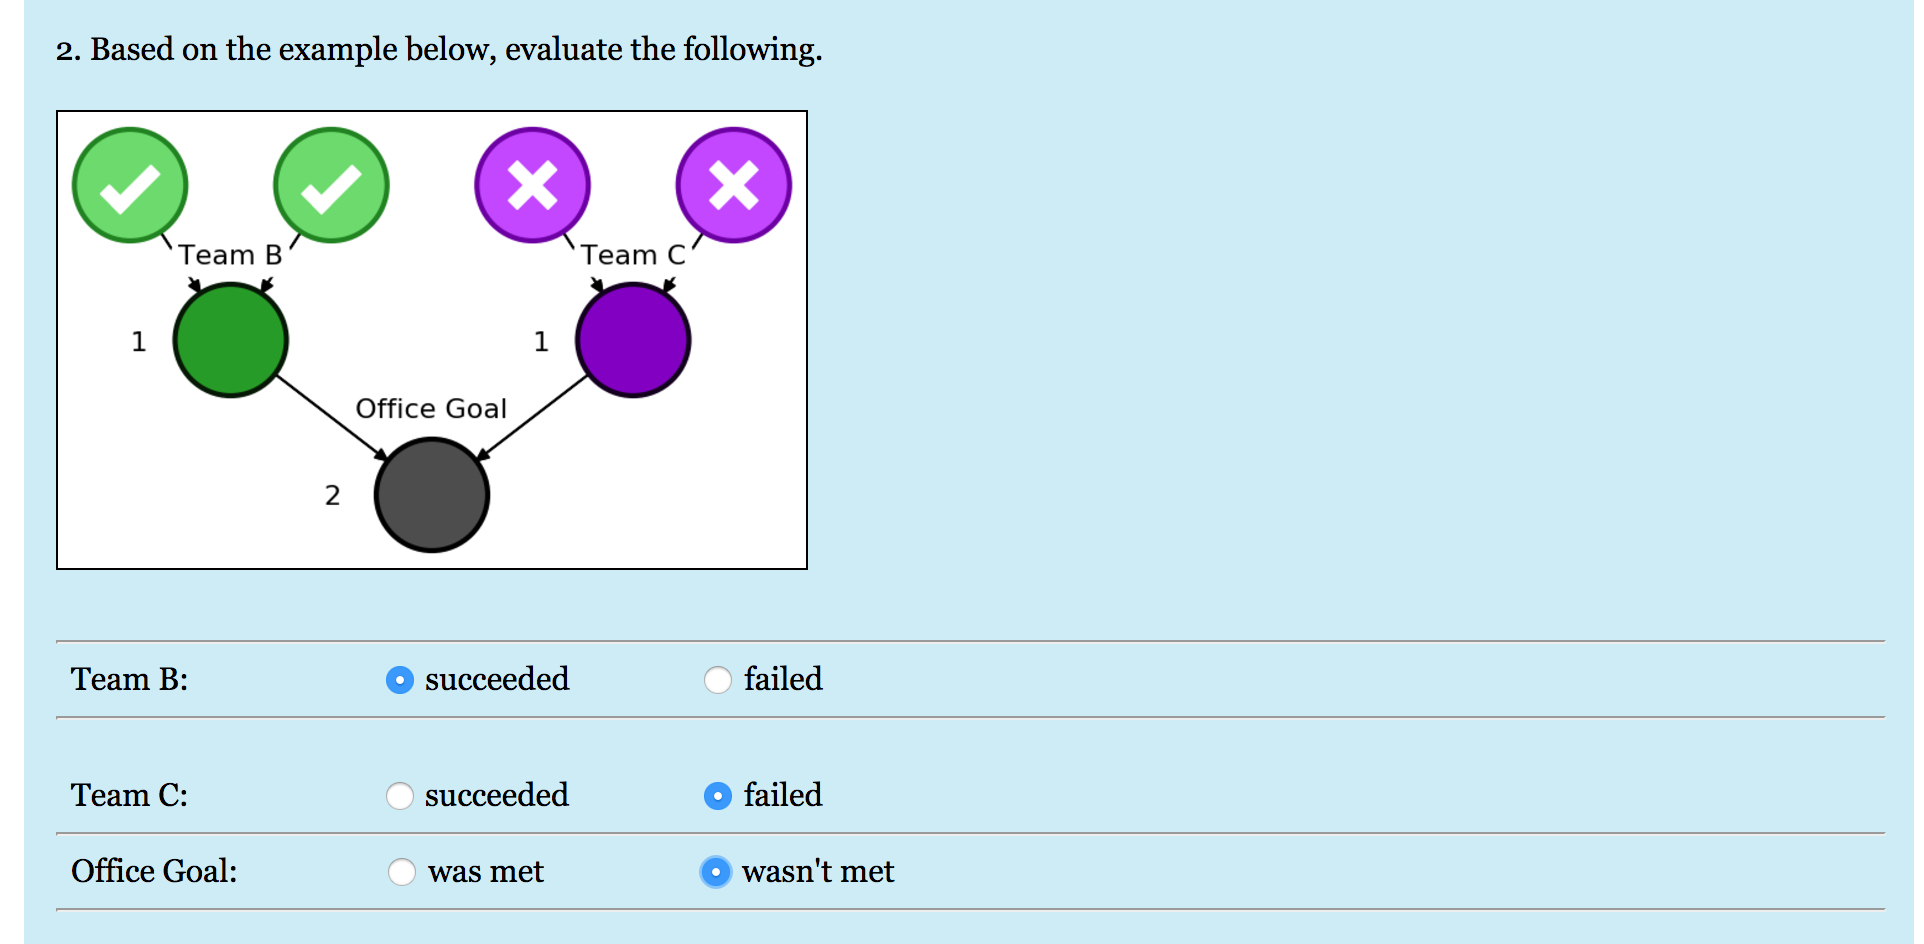
\includegraphics[width=0.95\textwidth]{screenshot_13}
	\caption{Instruction screenshot 13.}
	\label{fig:screenshot_13}
\end{figure}
\begin{figure}[H]
	\centering
	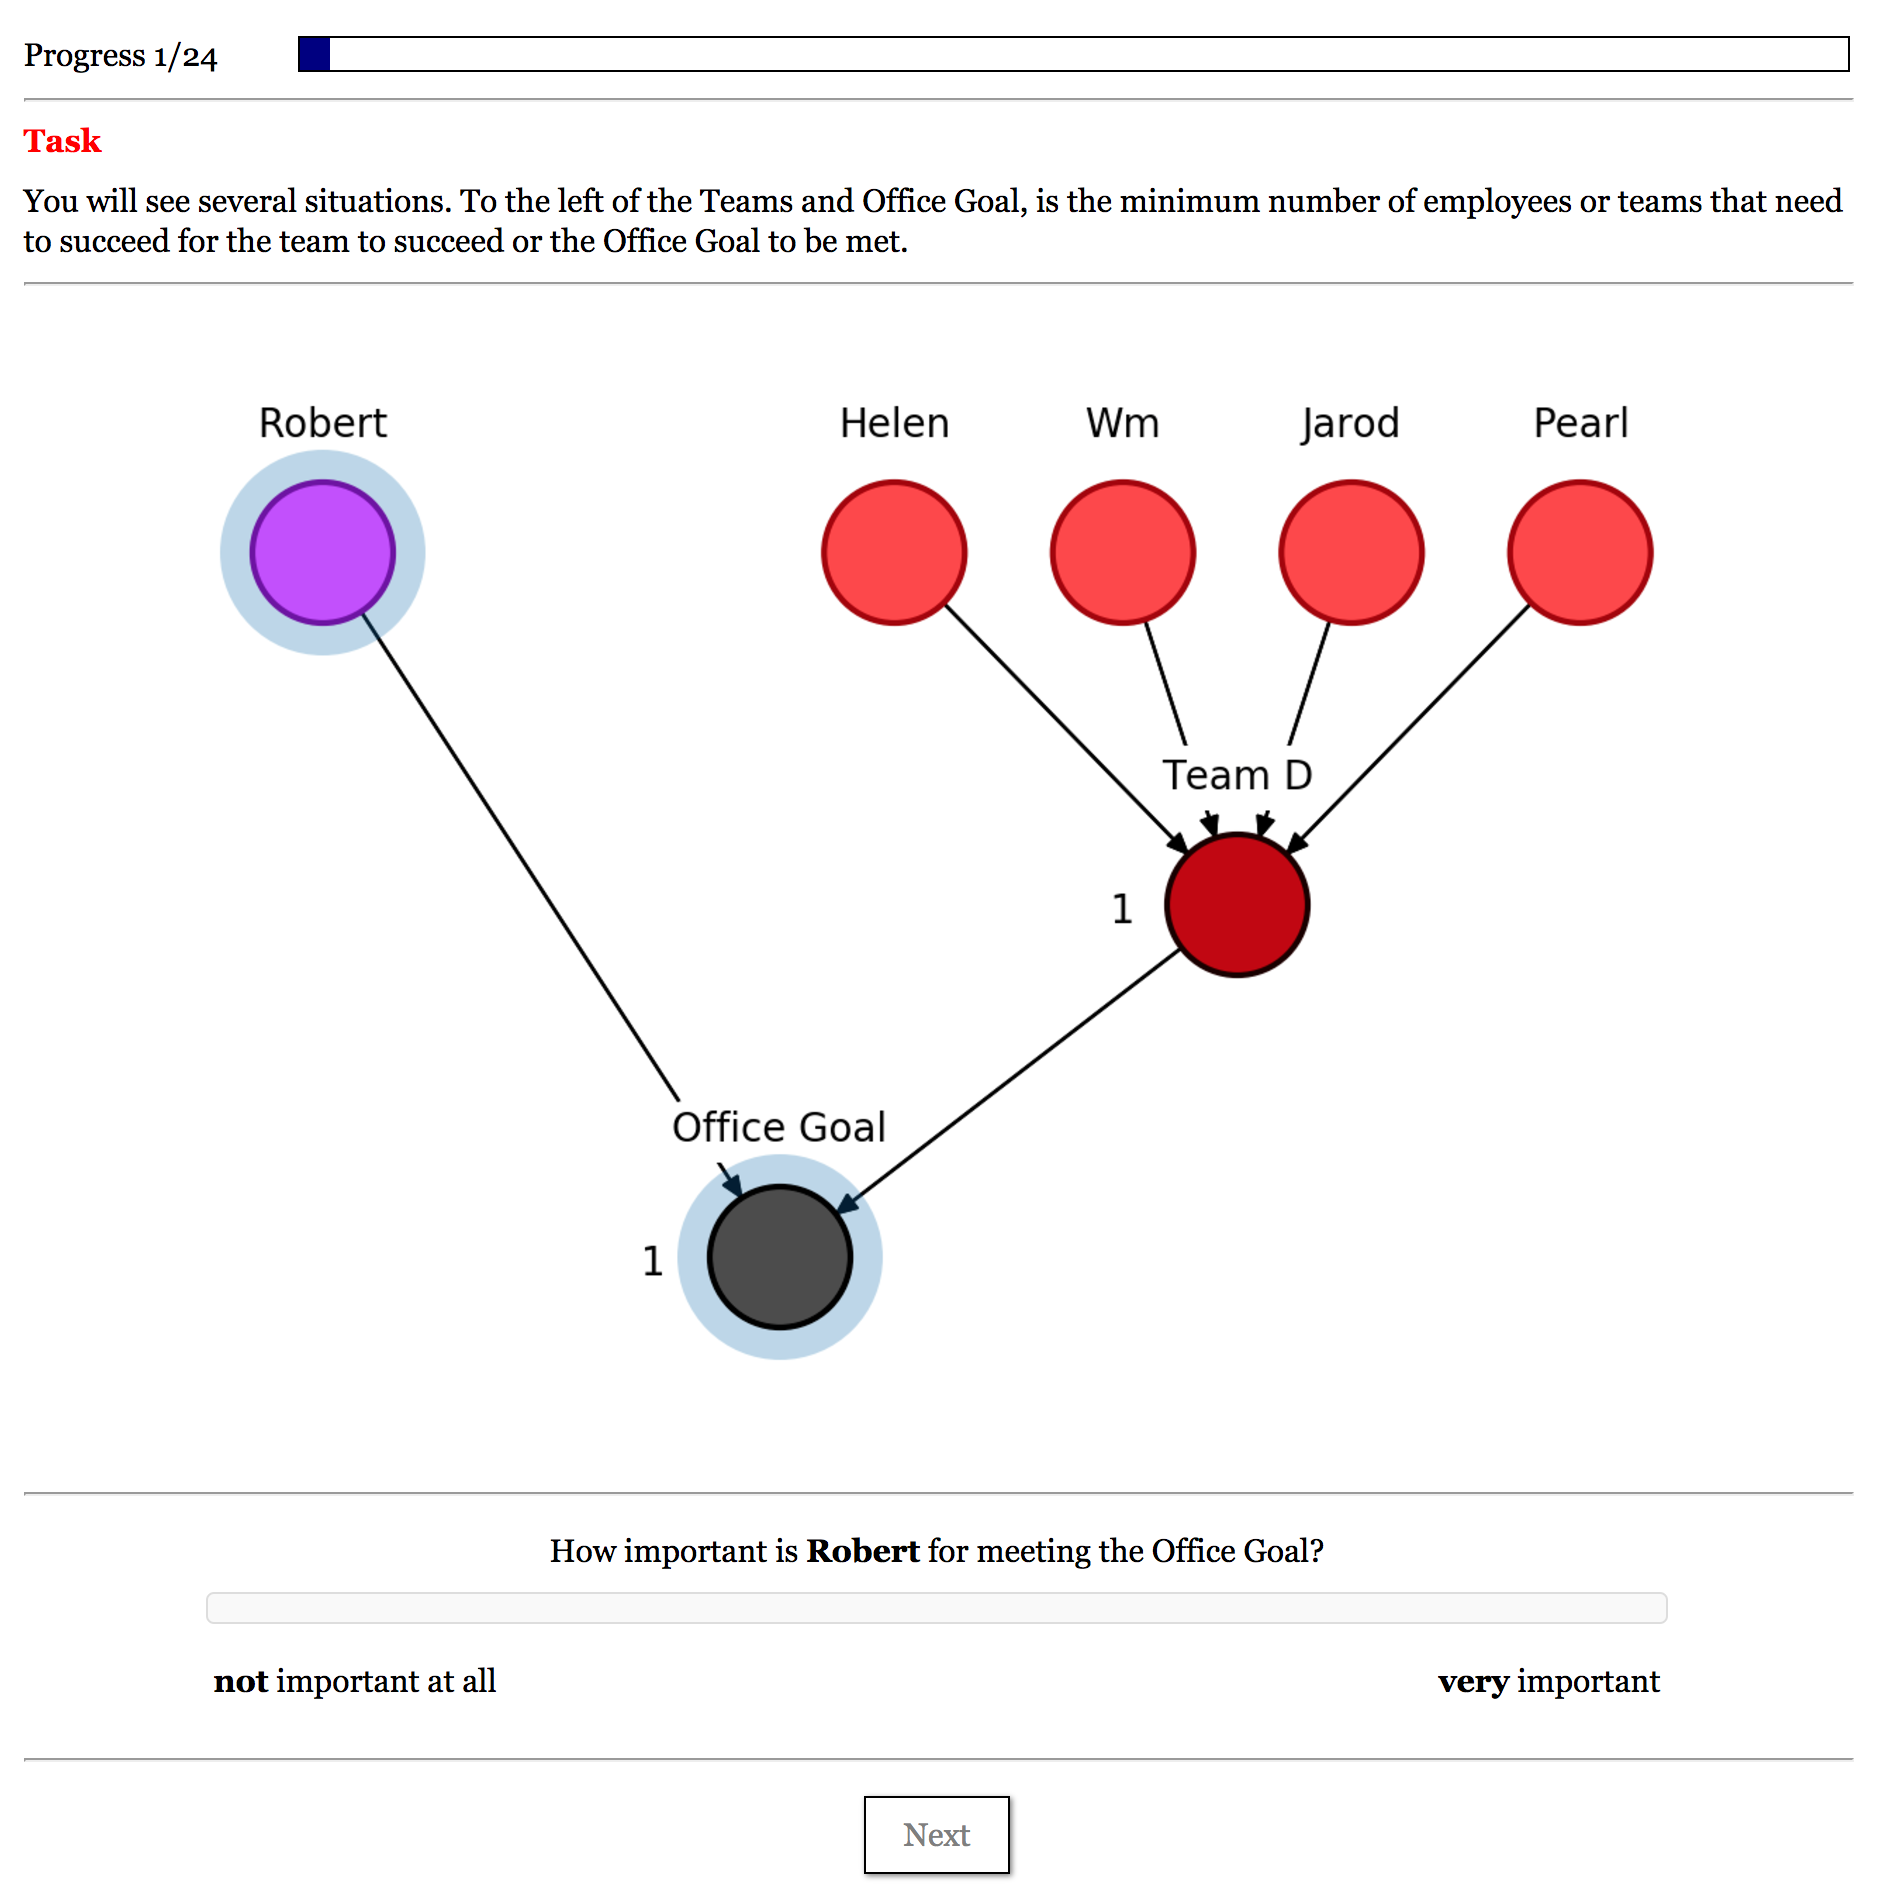
\includegraphics[width=0.95\textwidth]{screenshot_14}
	\caption{Instruction screenshot 14.}
	\label{fig:screenshot_14}
\end{figure}
\begin{figure}[H]
	\centering
	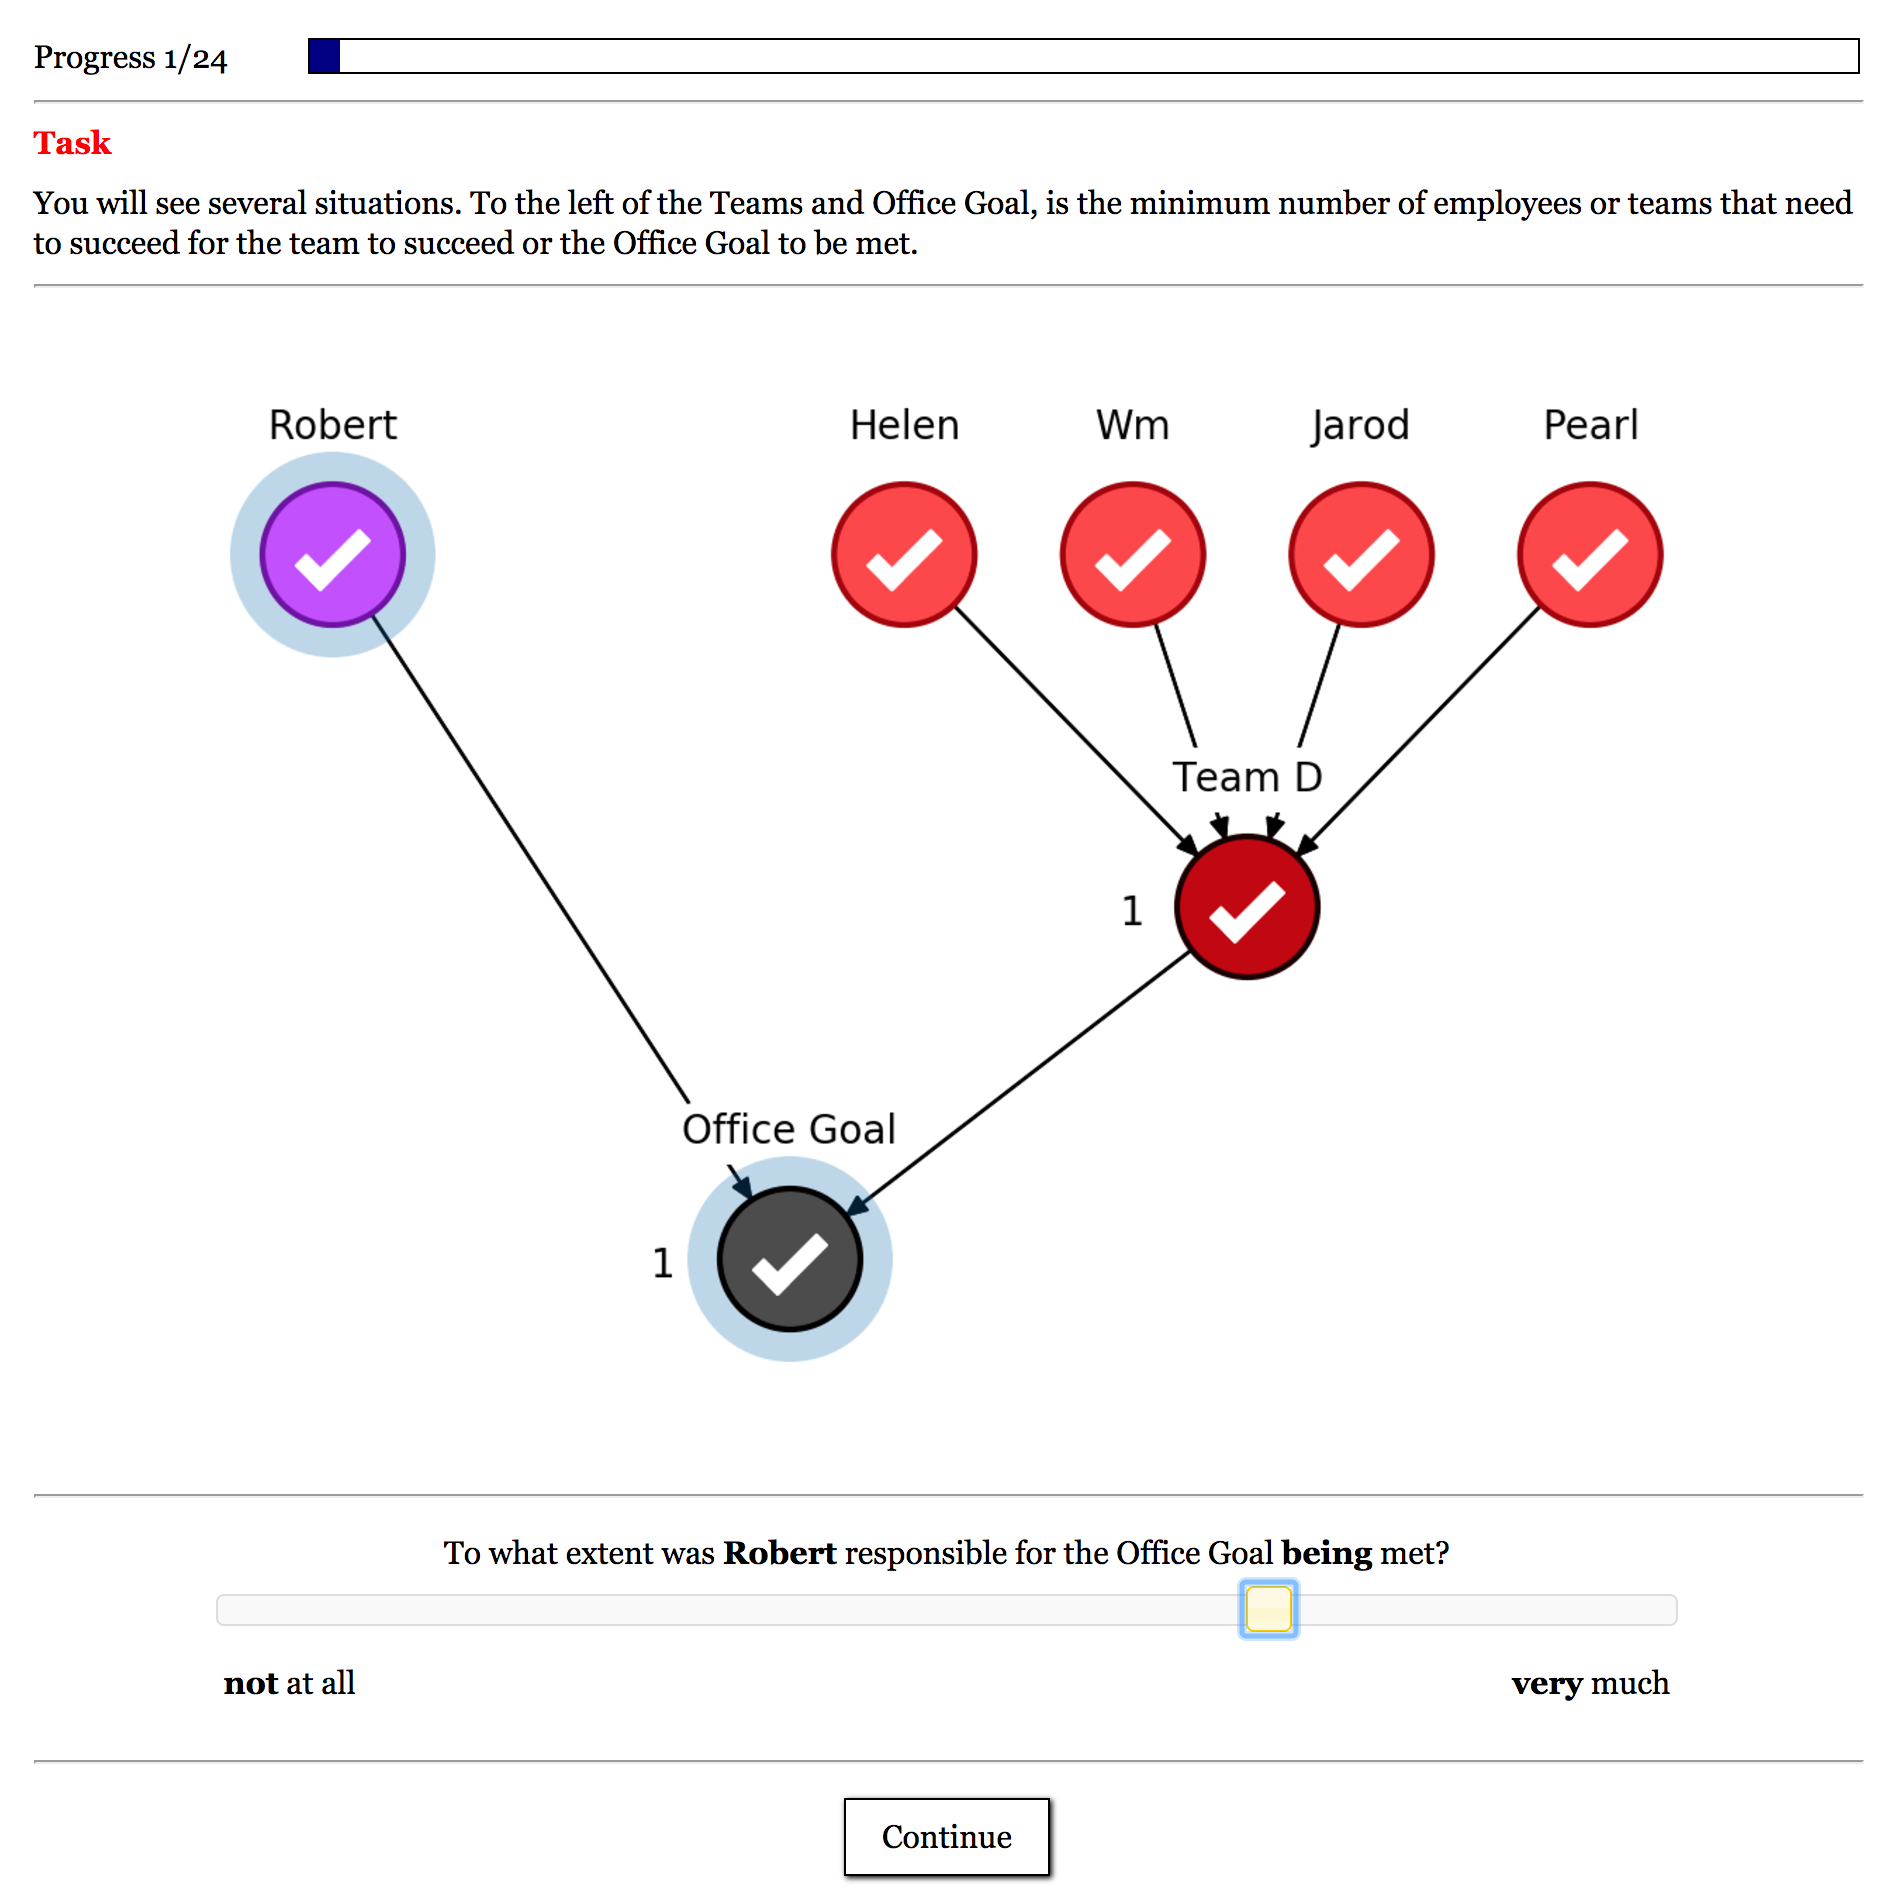
\includegraphics[width=0.95\textwidth]{screenshot_15}
	\caption{Instruction screenshot 15.}
	\label{fig:screenshot_15}
\end{figure}

\subsection{Results}
\label{sub:results}

\begin{figure}[H]
	\centering
	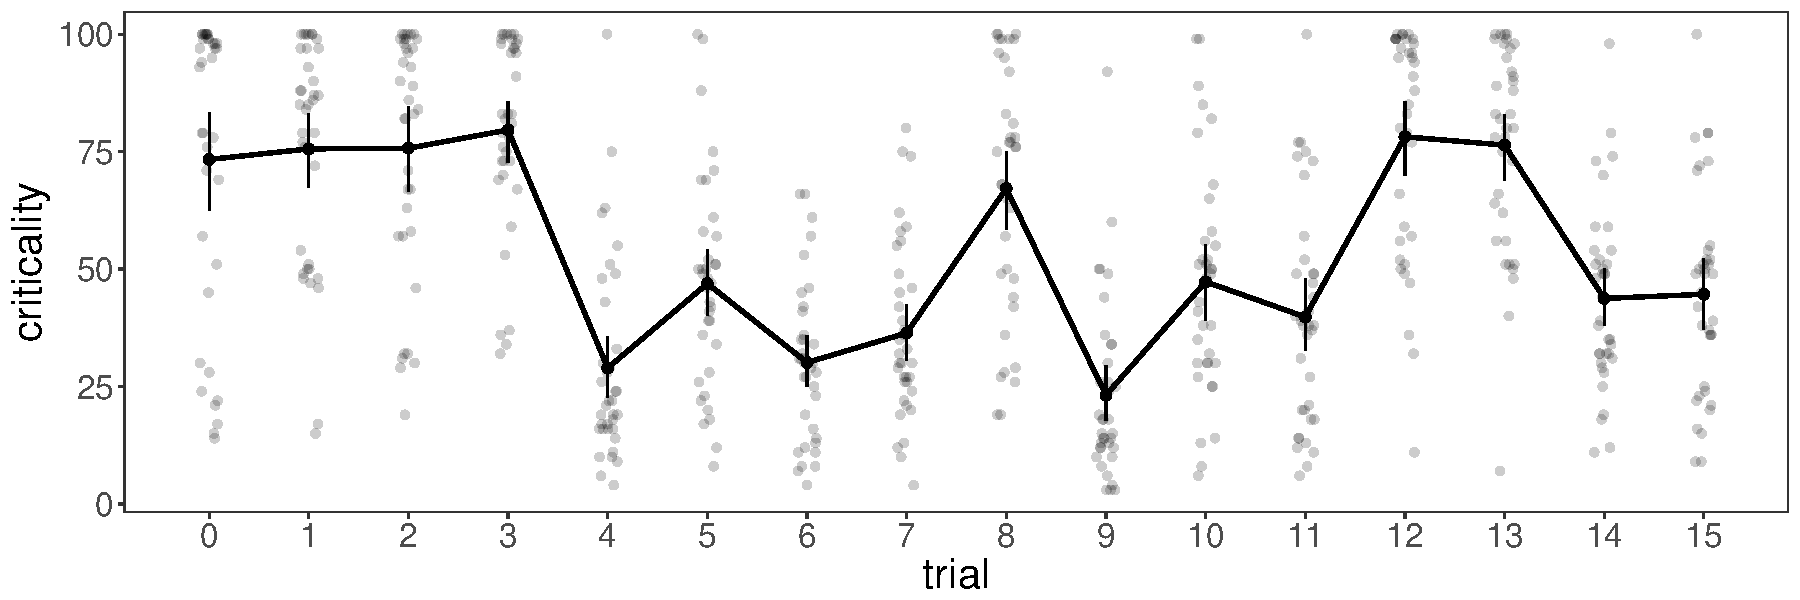
\includegraphics[width=0.95\textwidth]{criticality_judgments}
	\caption{Criticality judgments: ``How important is X for meeting the Office Goal?''}
	\label{fig:criticality_judgments}
\end{figure}

\begin{figure}[H]
	\centering
	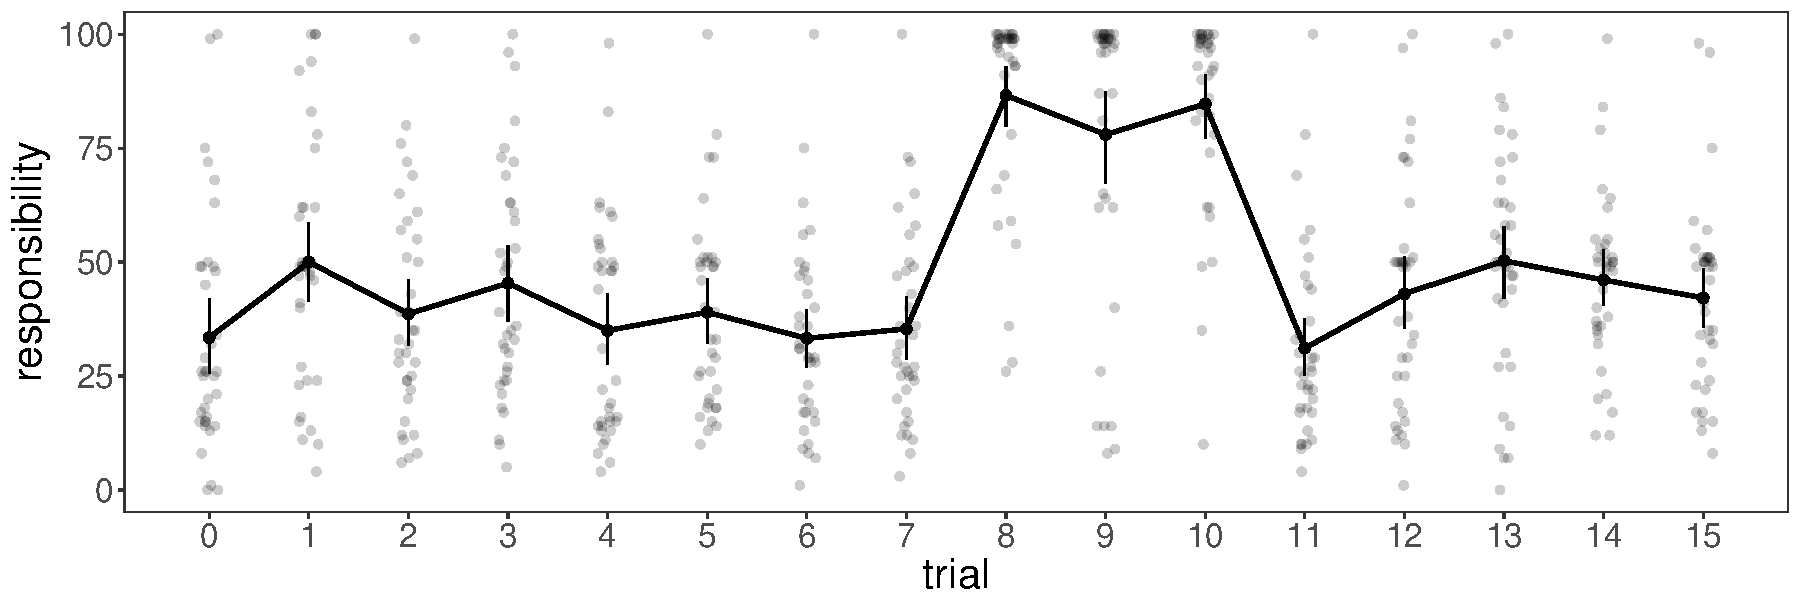
\includegraphics[width=0.95\textwidth]{responsibility_judgments}
	\caption{Responsibility judgments: ``To what extent was X responsible for the Office Goal [not] being met?''}
	\label{fig:responsibility_judgments}
\end{figure}

\subsection{Discussion}
\label{sub:discussion}

\end{document}